\documentclass[aspectratio=169]{beamer}
\usetheme{Madrid}
\usecolortheme{default}
\usepackage[utf8]{inputenc}
\usepackage[T5]{fontenc}
\usepackage{graphicx}
\usepackage{hyperref}
\usepackage{booktabs}
\usepackage{amsmath}
\usepackage{listings}
\usepackage{xcolor}

\setbeamertemplate{caption}[numbered]
\renewcommand{\figurename}{Hình}
\renewcommand{\thefigure}{11.\arabic{figure}}

% Cấu hình listings cho Python
\definecolor{codegreen}{rgb}{0,0.6,0}
\definecolor{codegray}{rgb}{0.5,0.5,0.5}
\definecolor{codepurple}{rgb}{0.58,0,0.82}
\definecolor{backcolour}{rgb}{0.95,0.95,0.92}

\lstdefinestyle{mystyle}{
    backgroundcolor=\color{backcolour},   
    commentstyle=\color{codegreen},
    keywordstyle=\color{magenta},
    numberstyle=\tiny\color{codegray},
    stringstyle=\color{codepurple},
    basicstyle=\ttfamily\scriptsize,
    breakatwhitespace=false,         
    breaklines=true,                 
    captionpos=b,                    
    keepspaces=true,                 
    numbers=left,                    
    numbersep=5pt,                  
    showspaces=false,                
    showstringspaces=false,
    showtabs=false,                  
    tabsize=2
}
\lstset{style=mystyle}

\title[Chương 11: Phân vùng Hình ảnh]{Học Sâu (Deep Learning) \\ \vspace{0.5cm} \Large Chương 11: Phân vùng Hình ảnh \\ (Image Segmentation)}
\author{Đại học Đông Á}
\date{\today}

\begin{document}

\begin{frame}
    \titlepage
\end{frame}

\begin{frame}{Nội dung chương}
    \tableofcontents
\end{frame}

\section{1. Tổng quan các Bài toán Thị giác Máy tính}

\begin{frame}{Ba nhánh chính của Thị giác Máy tính}
    \begin{columns}
        \column{0.4\textwidth}
        \begin{itemize}
            \item \textbf{Image Classification (Phân loại):} Gán nhãn cho toàn bộ bức ảnh ("Ảnh này có con mèo").
            \item \textbf{Object Detection (Phát hiện vật thể):} Vẽ hộp giới hạn (Bounding box) quanh vật thể và phân loại chúng ("Con mèo ở tọa độ x, y").
            \item \textbf{Image Segmentation (Phân vùng):} Phân loại ở cấp độ \textbf{Điểm ảnh (Pixel)}. Cắt chính xác đường viền của vật thể ("Những pixel nào thuộc về con mèo?").
        \end{itemize}
        
        \column{0.6\textwidth}
        \begin{figure}
            \centering
            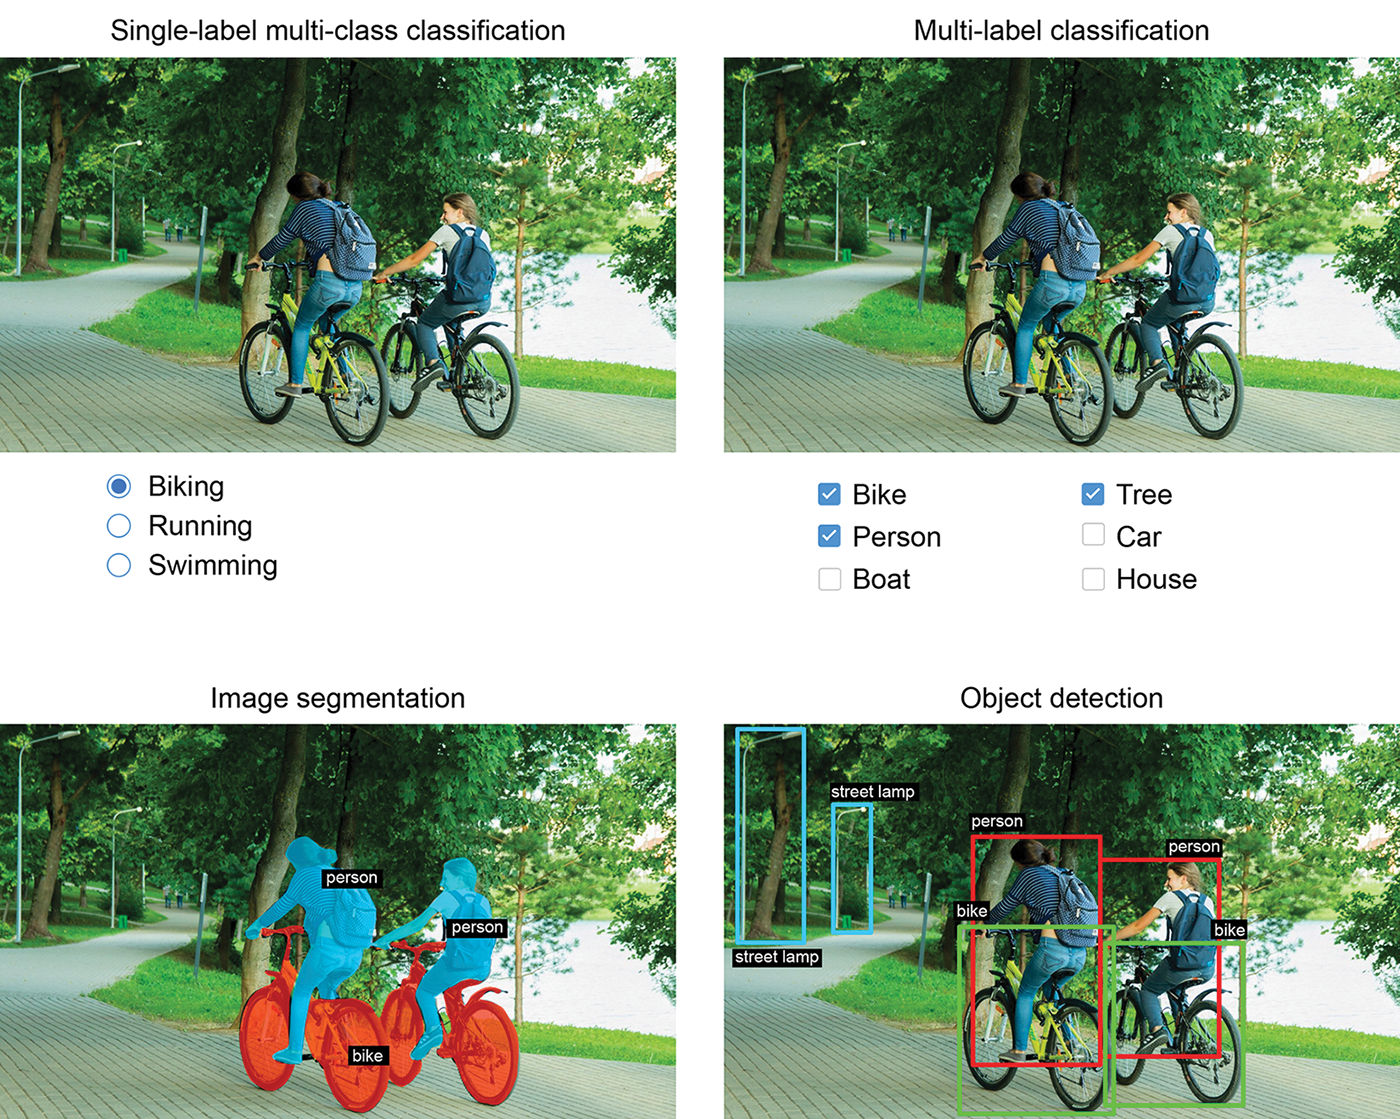
\includegraphics[width=\textwidth,height=0.6\textheight,keepaspectratio]{../../images/ch11/computer_vision_tasks.da2bf0ea.png}
            \caption{Ba bài toán cốt lõi trong CV}
        \end{figure}
    \end{columns}
\end{frame}

\begin{frame}{Phân loại Bài toán Image Segmentation}
    \begin{columns}
        \column{0.5\textwidth}
        \begin{itemize}
            \item \textbf{Semantic Segmentation:} Phân loại pixel theo "Danh mục" (Category). Nếu có 2 con mèo, cả 2 sẽ có cùng màu (cùng nhãn "Mèo").
            \item \textbf{Instance Segmentation:} Phân loại pixel theo "Cá thể" (Instance). Phân biệt rạch ròi "Con mèo 1" và "Con mèo 2".
            \item \textbf{Panoptic Segmentation:} Sự kết hợp cao cấp của cả Semantic và Instance Segmentation.
        \end{itemize}
        
        \column{0.5\textwidth}
        \begin{figure}
            \centering
            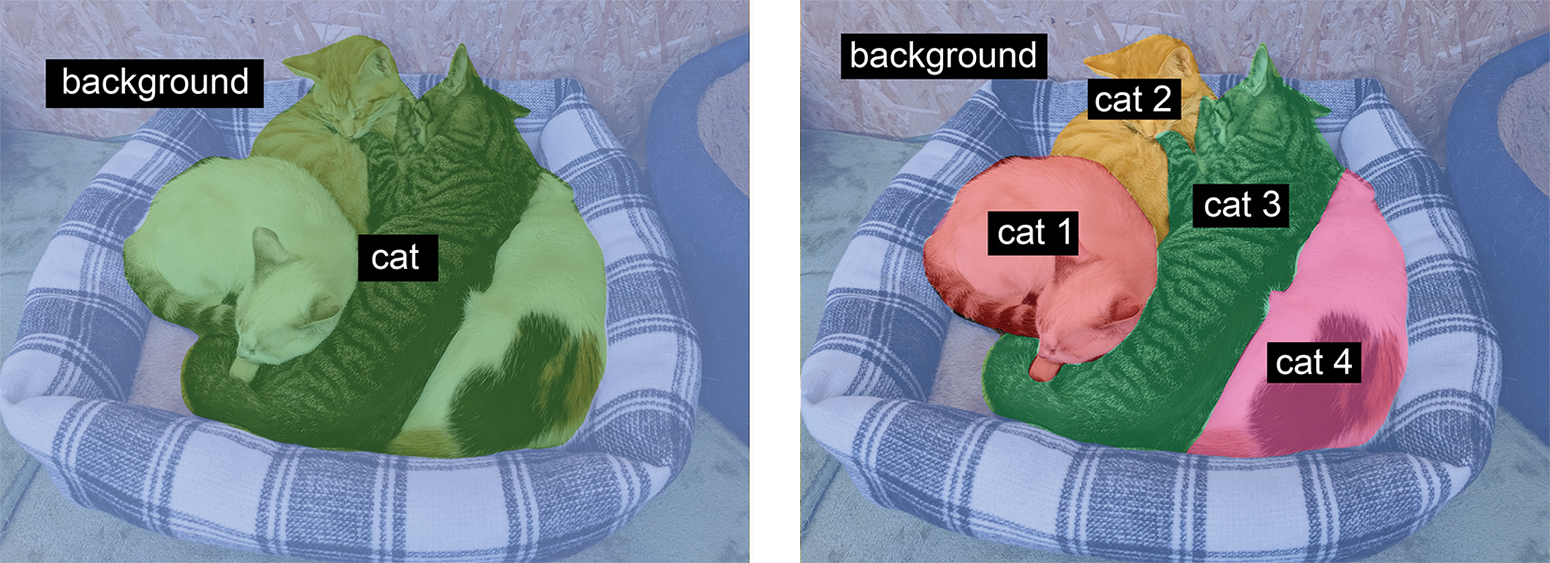
\includegraphics[width=\textwidth,height=0.6\textheight,keepaspectratio]{../../images/ch11/instance_segmentation.818c62ba.png}
            \caption{Semantic vs Instance Segmentation}
        \end{figure}
    \end{columns}
\end{frame}

\section{2. Xây dựng Mô hình Phân vùng Semantic}

\begin{frame}{Bài toán: Phân tách Tiền cảnh và Hậu cảnh}
    \begin{columns}
        \column{0.5\textwidth}
        \begin{itemize}
            \item Ta sẽ xây dựng một mô hình CNN từ đầu để thực hiện Semantic Segmentation trên tập dữ liệu Oxford-IIIT Pets (Chó \& Mèo).
            \item \textbf{Mục tiêu:} Phân biệt đâu là chủ thể (Vật nuôi), đâu là đường viền, và đâu là hậu cảnh (Background).
            \item Ảnh đầu vào: $200 \times 200 \times 3$.
        \end{itemize}
        
        \column{0.5\textwidth}
        \begin{figure}
            \centering
            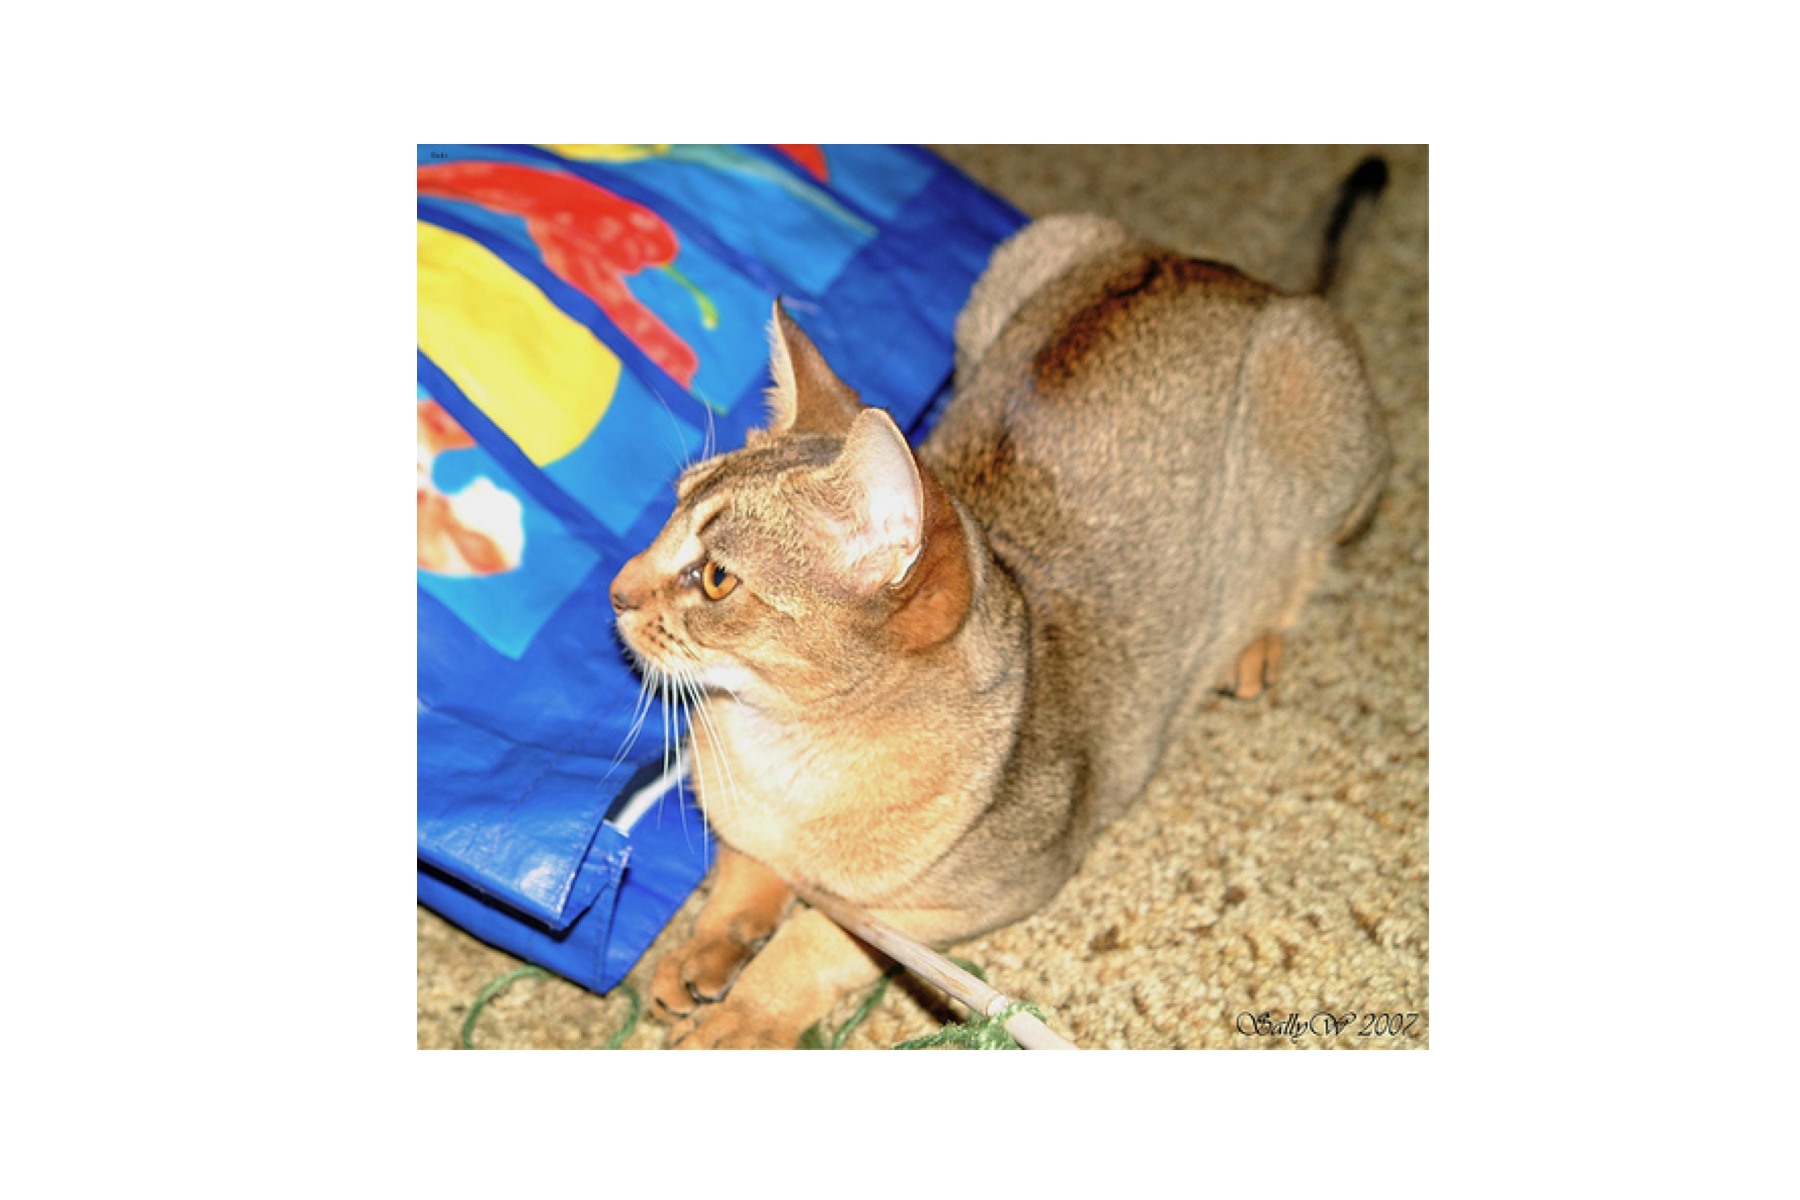
\includegraphics[width=\textwidth,height=0.6\textheight,keepaspectratio]{../../images/ch11/segmentation_input.d246cf5a.png}
            \caption{Ảnh đầu vào}
        \end{figure}
    \end{columns}
\end{frame}

\begin{frame}[fragile]{Tải Dữ liệu Oxford-IIIT Pets}
Sử dụng các lệnh \texttt{wget} và \texttt{tar} trên Colab để tải hình ảnh (images) và nhãn mặt nạ (annotations).

\begin{lstlisting}[language=bash]
!wget http://www.robots.ox.ac.uk/~vgg/data/pets/data/images.tar.gz
!wget http://www.robots.ox.ac.uk/~vgg/data/pets/data/annotations.tar.gz
!tar -xf images.tar.gz
!tar -xf annotations.tar.gz
\end{lstlisting}

Sắp xếp danh sách file (Xóa các file ẩn rác):

\begin{lstlisting}[language=Python]
import pathlib

input_dir = pathlib.Path("images")
target_dir = pathlib.Path("annotations/trimaps")

input_img_paths = sorted(input_dir.glob("*.jpg"))
# Ignores some spurious files in the trimaps directory that start with "."
target_paths = sorted(target_dir.glob("[!.]*.png"))
\end{lstlisting}
\end{frame}

\begin{frame}{Khái niệm Mặt nạ (Mask)}
    \begin{columns}
        \column{0.5\textwidth}
        \begin{itemize}
            \item Dữ liệu nhãn (Ground Truth) trong bài toán này không phải là một con số, mà là một \textbf{Mặt nạ (Mask)}.
            \item Kích thước Mask tương đương ảnh gốc ($200 \times 200 \times 1$).
            \item Mỗi pixel mang 1 trong 3 giá trị:
            \begin{enumerate}
                \item Foreground (Tiền cảnh)
                \item Background (Hậu cảnh)
                \item Contour (Đường viền)
            \end{enumerate}
        \end{itemize}
        
        \column{0.5\textwidth}
        \begin{figure}
            \centering
            
\includegraphics[width=\textwidth,height=0.6\textheight,keepaspectratio]{../../images/ch11/segmentation_mask.cc320651.png}
            \caption{Mặt nạ phân vùng (Ground truth)}
        \end{figure}
    \end{columns}
\end{frame}

\begin{frame}[fragile]{Hàm Load Ảnh và Mặt nạ}
Định nghĩa hàm đọc file từ ổ đĩa và chuyển thành Numpy array. Mặt nạ được xử lý thành thang xám (grayscale) và trừ 1 để đưa các nhãn về $[0, 1, 2]$.

\begin{lstlisting}[language=Python]
def path_to_input_image(path):
    return img_to_array(load_img(path, target_size=img_size))

def path_to_target(path):
    img = img_to_array(
        load_img(path, target_size=img_size, color_mode="grayscale")
    )
    # Subtracts 1 so that our labels become 0, 1, and 2
    img = img.astype("uint8") - 1
    return img
\end{lstlisting}
\end{frame}

\begin{frame}[fragile]{Nạp Hình ảnh vào mảng NumPy}
Khởi tạo hai mảng kích thước cực lớn chứa toàn bộ Data. Ảnh có 3 kênh màu, Mặt nạ chỉ có 1 kênh số nguyên.

\begin{lstlisting}[language=Python]
import numpy as np
import random
from keras.utils import load_img, img_to_array

img_size = (200, 200)
num_imgs = len(input_img_paths)

# Shuffles the file paths
random.Random(1337).shuffle(input_img_paths)
random.Random(1337).shuffle(target_paths)

input_imgs = np.zeros((num_imgs,) + img_size + (3,), dtype="float32")
targets = np.zeros((num_imgs,) + img_size + (1,), dtype="uint8")

# Loops over all elements to fill numpy arrays...
\end{lstlisting}
\end{frame}

\begin{frame}[fragile]{Chia tập Huấn luyện và Xác thực}
Tương tự bài toán phân loại ảnh, ta cần chia dữ liệu để tránh Overfitting.

\begin{lstlisting}[language=Python]
# Reserves 1,000 samples for validation
num_val_samples = 1000

# Splits the data into a training and a validation set
train_input_imgs = input_imgs[:-num_val_samples]
train_targets = targets[:-num_val_samples]

val_input_imgs = input_imgs[-num_val_samples:]
val_targets = targets[-num_val_samples:]
\end{lstlisting}
Dù kích thước tập dữ liệu tương đối nhỏ (hơn 7000 ảnh), nhưng nhờ kỹ thuật Data Augmentation và kiến trúc CNN mạnh, ta vẫn có thể học tốt.
\end{frame}

\begin{frame}{Kiến trúc Encoder - Decoder (U-Net style)}
    Mạng nơ-ron phân vùng có hình phễu, chia làm 2 nửa:
    \begin{itemize}
        \item \textbf{Encoder (Mã hóa):} Dùng \texttt{Conv2D} với \texttt{strides=2} để \textbf{Hạ độ phân giải} ảnh xuống (Ví dụ: $200 \rightarrow 100 \rightarrow 50$). Nhằm trích xuất thông tin khái niệm (What).
        \item \textbf{Decoder (Giải mã):} Dùng \texttt{Conv2DTranspose} với \texttt{strides=2} để \textbf{Tăng độ phân giải} ảnh lên lại (Ví dụ: $50 \rightarrow 100 \rightarrow 200$). Nhằm định vị lại không gian gốc (Where).
    \end{itemize}
\end{frame}

\begin{frame}{Toán học của Transposed Convolution}
    \begin{itemize}
        \item Để tăng độ phân giải (Upsampling) mà vẫn duy trì khả năng học hỏi (Learnable), ta dùng \textbf{Tích chập Chuyển vị (Transposed Convolution)}.
        \item Nó hoạt động ngược lại với Tích chập thông thường:
        \begin{itemize}
            \item Nhận 1 giá trị đầu vào (Pixel).
            \item Nhân giá trị đó với một Bộ lọc (Kernel).
            \item Phát tán (Broadcast) kết quả ra một vùng không gian lớn hơn ở đầu ra.
        \end{itemize}
        \item Nhờ đó, mạng có thể học cách "điền" thông tin chi tiết vào những vùng ảnh đã bị thu nhỏ trước đó.
    \end{itemize}
\end{frame}

\begin{frame}[fragile]{Định nghĩa Nửa thứ nhất - Encoder}
Hạ độ phân giải ảnh để nén đặc trưng. Lưu ý ta dùng \texttt{strides=2} thay cho MaxPooling để giữ lại thông tin tọa độ không gian (Location info).

\begin{lstlisting}[language=Python]
import keras
from keras.layers import Rescaling, Conv2D, Conv2DTranspose

def get_model(img_size, num_classes):
    inputs = keras.Input(shape=img_size + (3,))
    x = Rescaling(1.0 / 255)(inputs)

    # Encoder part: Downsampling
    x = Conv2D(64, 3, strides=2, activation="relu", padding="same")(x)
    x = Conv2D(64, 3, activation="relu", padding="same")(x)
    x = Conv2D(128, 3, strides=2, activation="relu", padding="same")(x)
    x = Conv2D(128, 3, activation="relu", padding="same")(x)
    x = Conv2D(256, 3, strides=2, padding="same", activation="relu")(x)
    x = Conv2D(256, 3, activation="relu", padding="same")(x)
\end{lstlisting}
\end{frame}

\begin{frame}[fragile]{Định nghĩa Nửa thứ hai - Decoder}
Sử dụng \texttt{Conv2DTranspose} khôi phục lại độ phân giải $200 \times 200$ ban đầu. Output cuối cùng có $3$ kênh (tương ứng 3 class) với Softmax.

\begin{lstlisting}[language=Python]
    # Decoder part: Upsampling
    x = Conv2DTranspose(256, 3, activation="relu", padding="same")(x)
    x = Conv2DTranspose(256, 3, strides=2, activation="relu", padding="same")(x)
    x = Conv2DTranspose(128, 3, activation="relu", padding="same")(x)
    x = Conv2DTranspose(128, 3, strides=2, activation="relu", padding="same")(x)
    x = Conv2DTranspose(64, 3, activation="relu", padding="same")(x)
    x = Conv2DTranspose(64, 3, strides=2, activation="relu", padding="same")(x)

    # Ends with per-pixel softmax classifier
    outputs = Conv2D(num_classes, 3, activation="softmax", padding="same")(x)
    return keras.Model(inputs, outputs)

model = get_model(img_size=img_size, num_classes=3)
\end{lstlisting}
\end{frame}

\begin{frame}[fragile]{Độ đo IoU (Intersection over Union)}
IoU đo phần trăm giao nhau giữa Mặt nạ thực tế và Mặt nạ dự đoán. IoU = Giao / Hợp (Nằm trong khoảng 0-1).

\begin{lstlisting}[language=Python]
foreground_iou = keras.metrics.IoU(
    # Specifies the total number of classes
    num_classes=3,
    # Specifies the class to compute IoU for (0 = foreground)
    target_class_ids=(0,),
    name="foreground_iou",
    # Our targets are sparse (integer class IDs).
    sparse_y_true=True,
    # But our model predictions are a dense softmax!
    sparse_y_pred=False,
)
\end{lstlisting}
\end{frame}

\begin{frame}{Biểu đồ Loss trong Huấn luyện}
    \begin{columns}
        \column{0.5\textwidth}
        \begin{itemize}
            \item Vì đây là phân loại 3 nhãn cho từng pixel, ta dùng Hàm mất mát: \texttt{sparse\_categorical\_crossentropy}.
            \item Mô hình hội tụ rất tốt ở giai đoạn đầu.
            \item Bắt đầu xuất hiện Overfitting sau epoch thứ 25.
        \end{itemize}
        
        \column{0.5\textwidth}
        \begin{figure}
            \centering
            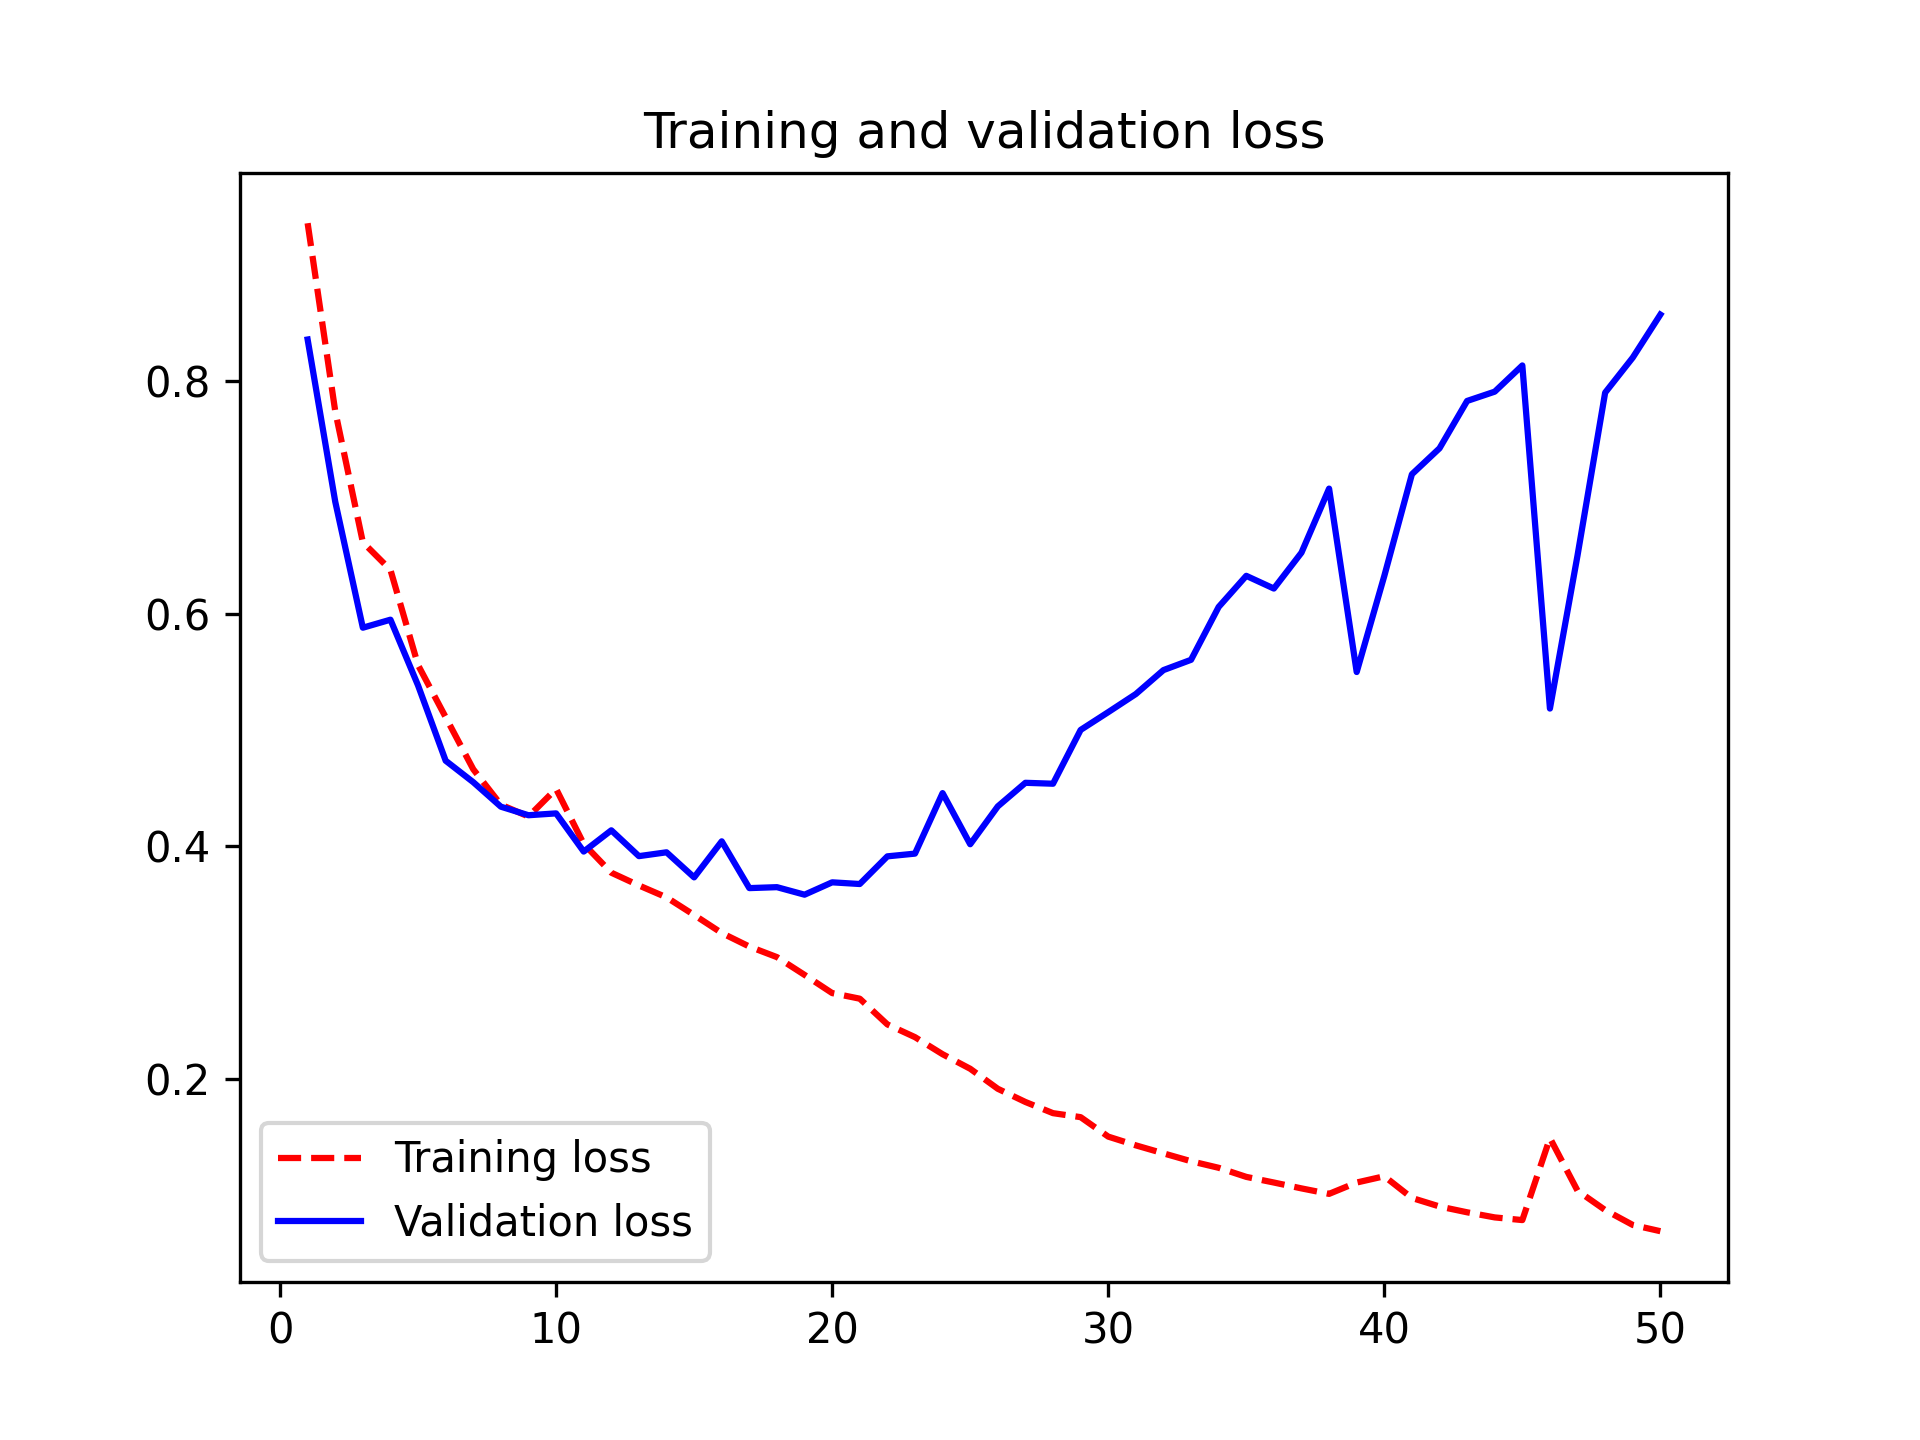
\includegraphics[width=\textwidth,height=0.6\textheight,keepaspectratio]{../../images/ch11/segmentation_loss.489fa0c8.png}
            \caption{Quá trình Training Loss}
        \end{figure}
    \end{columns}
\end{frame}

\begin{frame}[fragile]{Biên dịch và Huấn luyện (Train)}

\begin{lstlisting}[language=Python]
model.compile(
    optimizer="adam",
    loss="sparse_categorical_crossentropy",
    metrics=[foreground_iou],
)

callbacks = [
    keras.callbacks.ModelCheckpoint(
        "oxford_segmentation.keras", save_best_only=True
    )
]

history = model.fit(
    train_input_imgs, train_targets,
    epochs=50, batch_size=64,
    callbacks=callbacks,
    validation_data=(val_input_imgs, val_targets),
)
\end{lstlisting}
\end{frame}

\begin{frame}{Kết quả Dự đoán (Prediction)}
    \begin{columns}
        \column{0.5\textwidth}
        \begin{itemize}
            \item Trực quan hóa kết quả dự đoán của mô hình tự thiết kế.
            \item Mô hình bắt được hình dáng của con mèo khá tốt (Khu vực Tiền cảnh).
            \item Tuy nhiên, các chi tiết nhỏ ở đường viền (như tai, râu) vẫn còn nhiễu và bị mờ (Artifacts).
            \item Để đạt độ chính xác SOTA, ta cần các mô hình lớn hơn rất nhiều.
        \end{itemize}
        
        \column{0.5\textwidth}
        \begin{figure}
            \centering
            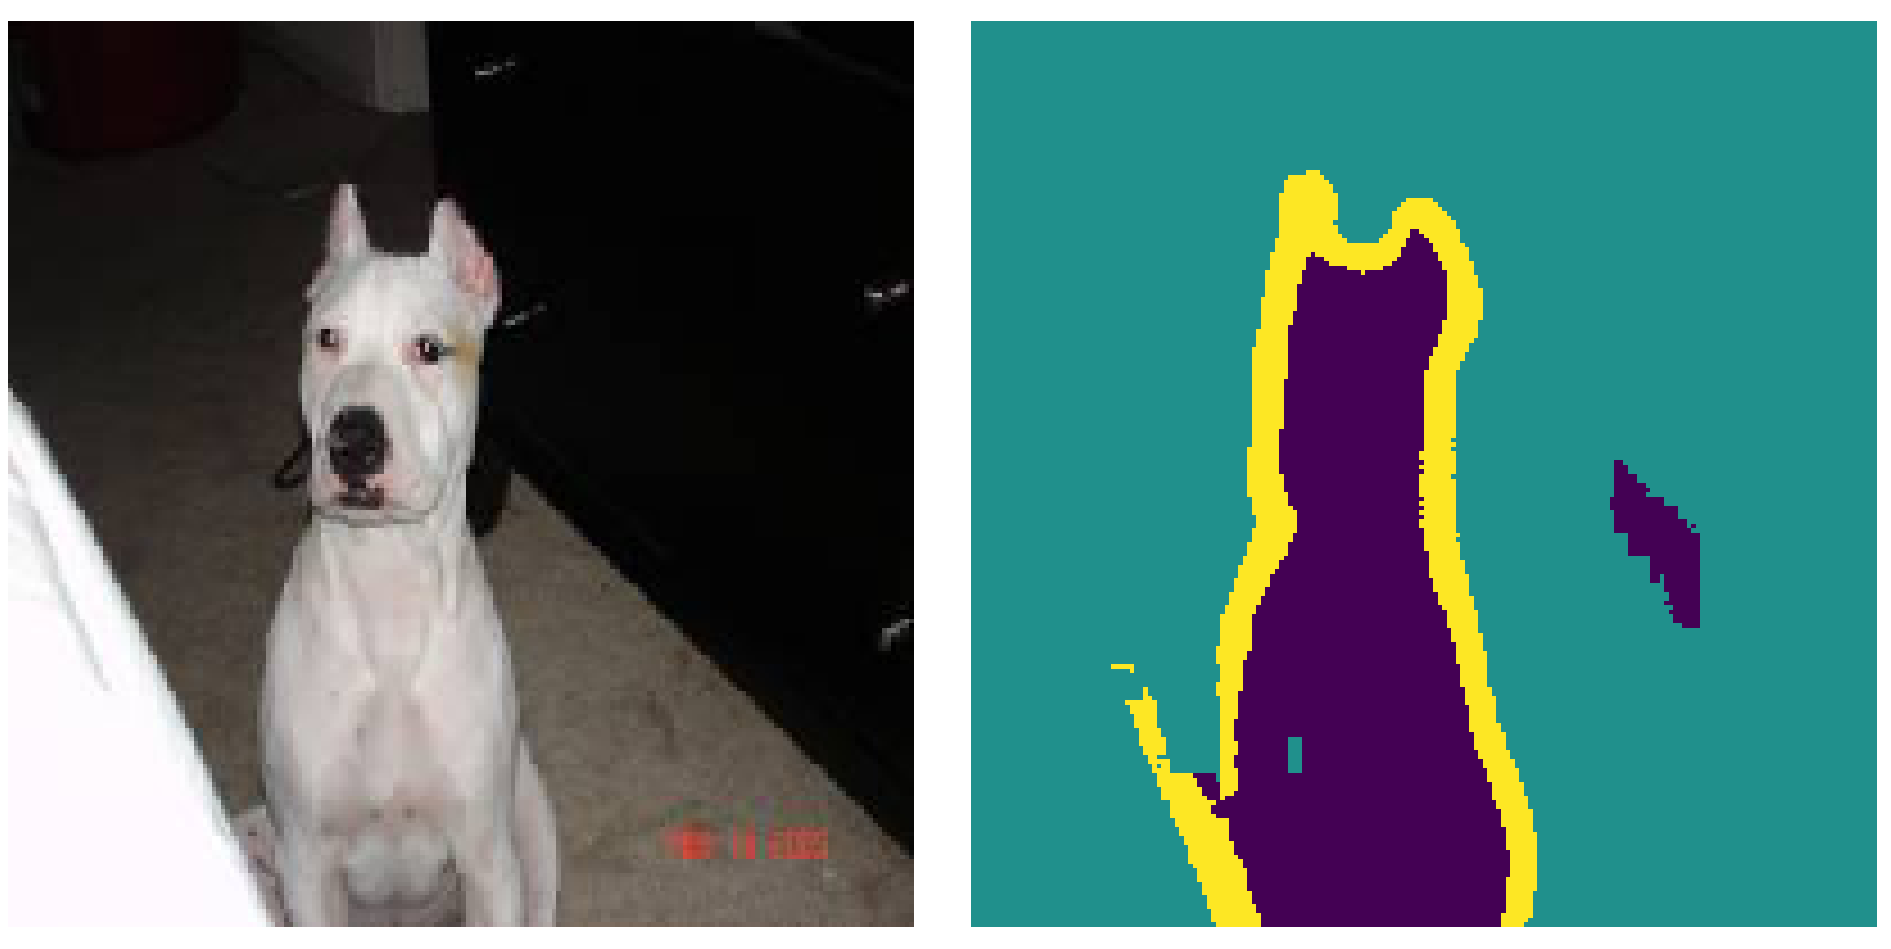
\includegraphics[width=\textwidth,height=0.6\textheight,keepaspectratio]{../../images/ch11/segmentation_test.ece7f638.png}
            \caption{Mặt nạ do mô hình dự đoán}
        \end{figure}
    \end{columns}
\end{frame}

\section{3. Siêu mô hình Nền tảng: Segment Anything (SAM)}

\begin{frame}{Kỷ nguyên của Foundation Models trong CV}
    \begin{itemize}
        \item Natural Language Processing (NLP) đã thay đổi mãi mãi với sự xuất hiện của các Foundation Models (Như GPT-3, GPT-4) - Một mô hình huấn luyện một lần, giải quyết được mọi tác vụ (Zero-shot).
        \item Vào tháng 4/2023, Meta AI công bố \textbf{Segment Anything Model (SAM)}, đánh dấu cột mốc Foundation Model đầu tiên của ngành Thị giác Máy tính (Computer Vision).
        \item SAM có khả năng phân vùng "Bất cứ thứ gì" trong ảnh, mà không cần huấn luyện lại.
    \end{itemize}
\end{frame}

\begin{frame}{Kiến trúc của SAM}
    \begin{columns}
        \column{0.5\textwidth}
        SAM gồm 3 thành phần cốt lõi:
        \begin{enumerate}
            \item \textbf{Image Encoder:} Vision Transformer (ViT) kích thước cực lớn, giải nén toàn bộ thông tin ảnh.
            \item \textbf{Prompt Encoder:} Biểu diễn các Lệnh nhắc của người dùng (Điểm, Hộp, Text).
            \item \textbf{Mask Decoder:} Một mạng nhẹ hợp nhất thông tin từ Image và Prompt để xuất ra Mặt nạ (Mask).
        \end{enumerate}
        
        \column{0.5\textwidth}
        \begin{figure}
            \centering
            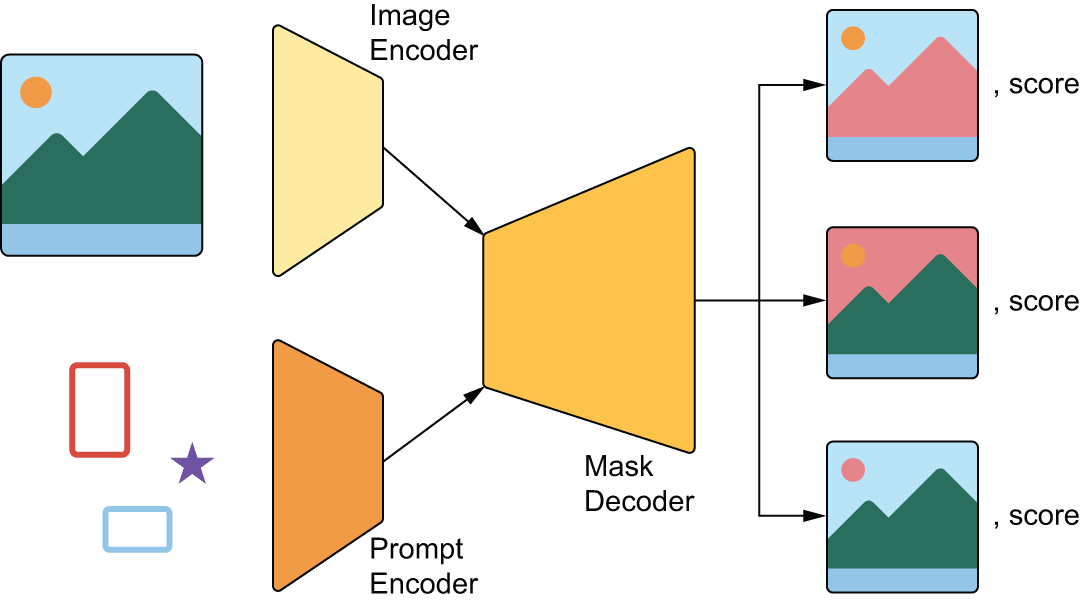
\includegraphics[width=\textwidth,height=0.5\textheight,keepaspectratio]{../../images/ch11/sam_architecture.dad9dae6.png}
            \caption{Kiến trúc tổng thể của Segment Anything}
        \end{figure}
    \end{columns}
\end{frame}

\begin{frame}{Siêu Dữ liệu SA-1B}
    \begin{columns}
        \column{0.5\textwidth}
        \begin{itemize}
            \item Sức mạnh của SAM đến từ Dữ liệu. Meta AI đã xây dựng tập dữ liệu \textbf{SA-1B (Segment Anything 1-Billion)}.
            \item Khối lượng khổng lồ: \textbf{11 triệu hình ảnh} với hơn \textbf{1.1 Tỷ mặt nạ phân vùng} chất lượng cao (gấp 400 lần các tập dữ liệu trước đó).
            \item Nhờ vậy, SAM có khả năng phân vùng Zero-shot với mọi thể loại vật thể từ sinh học, phương tiện, đến y tế.
        \end{itemize}
        
        \column{0.5\textwidth}
        \begin{figure}
            \centering
            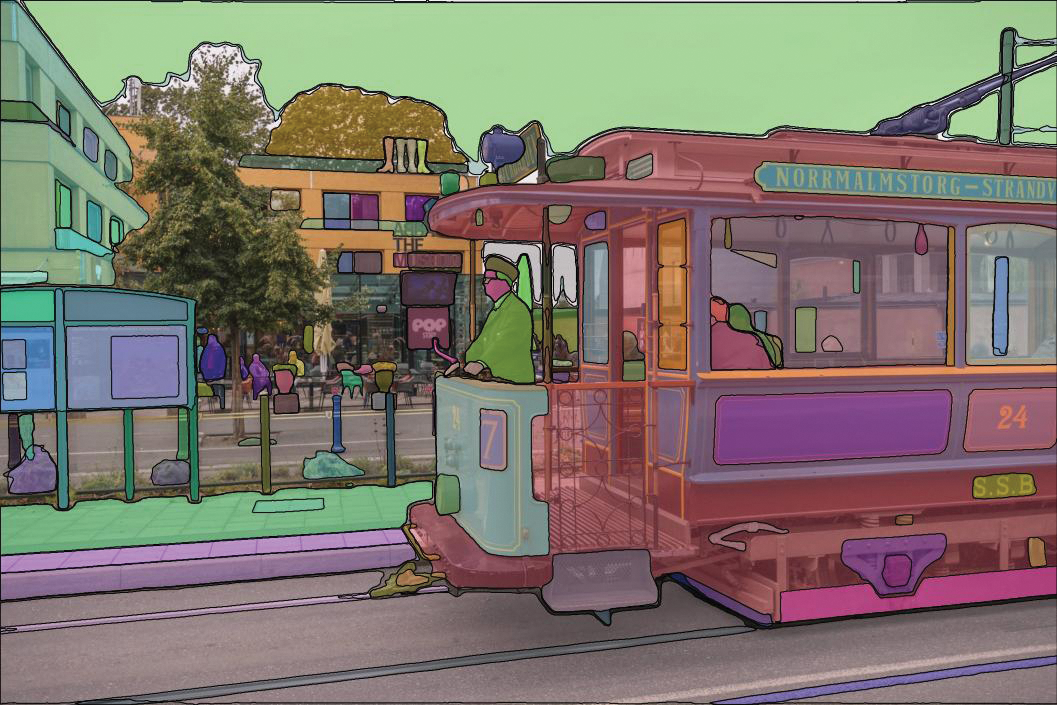
\includegraphics[width=\textwidth,height=0.6\textheight,keepaspectratio]{../../images/ch11/sa1b_example.6701768b.jpg}
            \caption{Mật độ mặt nạ trong tập dữ liệu SA-1B}
        \end{figure}
    \end{columns}
\end{frame}

\begin{frame}[fragile]{Khởi tạo SAM từ KerasHub}
Mọi thứ đều có sẵn trong KerasHub, ta gọi mô hình siêu lớn với Preset \texttt{sam\_huge\_sa1b}.

\begin{lstlisting}[language=Python]
import keras_hub

# Instantiates SAM and downloads its weights
model = keras_hub.models.ImageSegmenter.from_preset("sam_huge_sa1b")

print(model.count_params())
# Output: 641090864
\end{lstlisting}

Với 641 triệu tham số, đây là mô hình lớn nhất mà chúng ta sử dụng! Tốc độ tiến hóa của Pre-trained Models tỷ lệ thuận với lượng dữ liệu cung cấp (Sẽ học ở Chương 16).
\end{frame}

\section{4. Thực hành Kỹ nghệ Prompting trên SAM}

\begin{frame}{Môi trường Thử nghiệm}
    \begin{columns}
        \column{0.5\textwidth}
        \begin{itemize}
            \item Ta sẽ thử nghiệm sức mạnh của SAM trên một bức ảnh thực tế chứa rất nhiều loại Trái cây (Chuối, Đào, Xoài).
            \item Bức ảnh này có cấu trúc phức tạp với vật thể chồng chéo và bóng đổ.
            \item Mục tiêu: Gọi API của SAM để phân vùng chúng thông qua các kiểu \textbf{Prompting (Lệnh nhắc)} khác nhau.
        \end{itemize}
        
        \column{0.5\textwidth}
        \begin{figure}
            \centering
            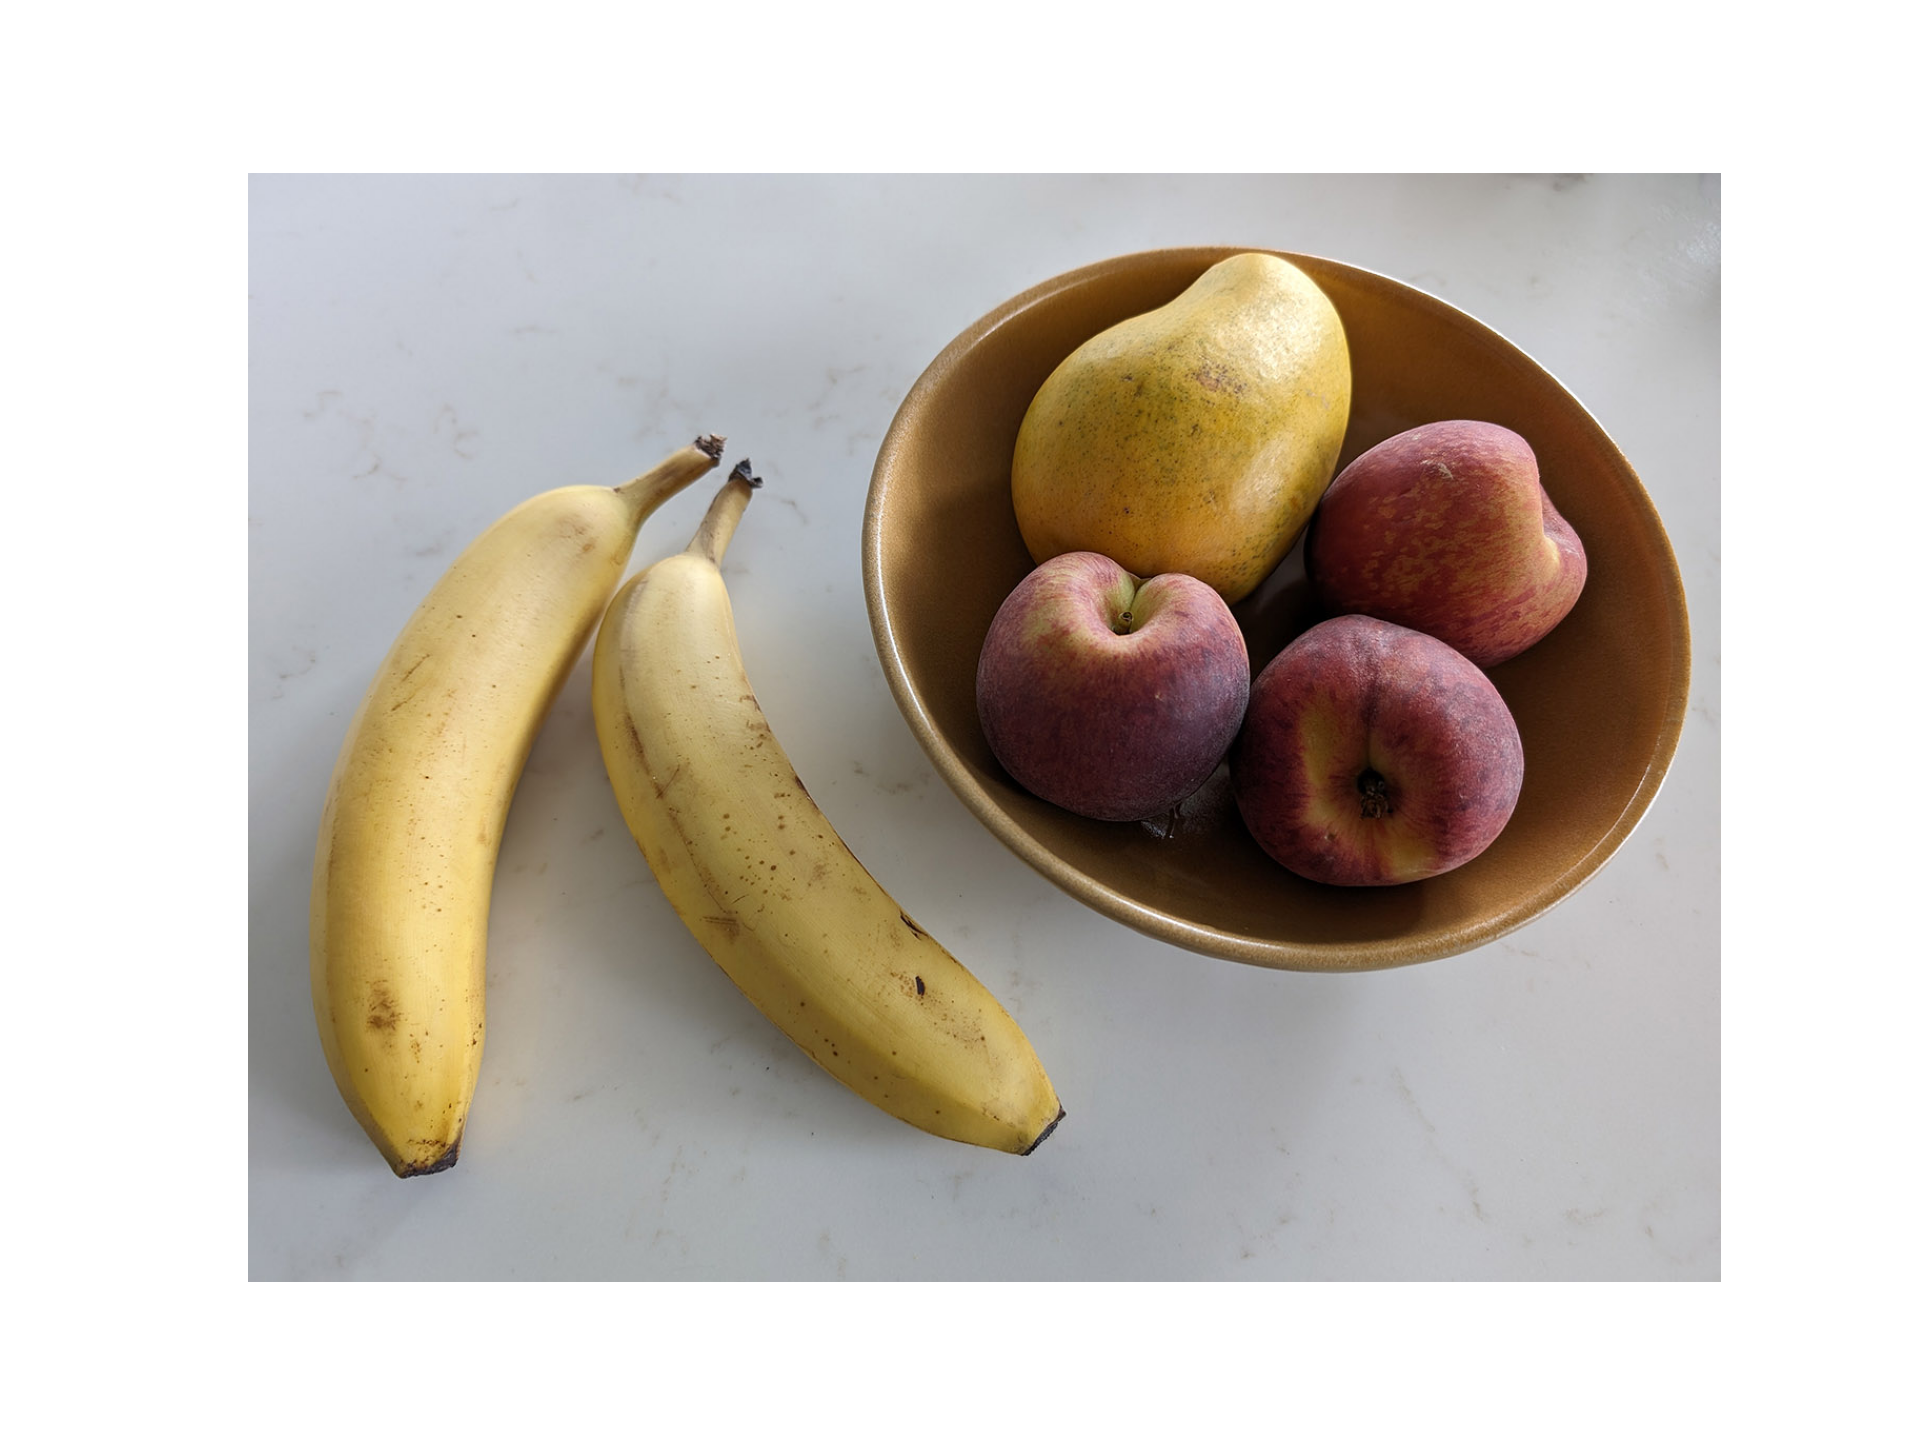
\includegraphics[width=\textwidth,height=0.6\textheight,keepaspectratio]{../../images/ch11/fruits.8cef44dc.png}
            \caption{Ảnh Trái cây đầu vào}
        \end{figure}
    \end{columns}
\end{frame}

\begin{frame}[fragile]{Tiền xử lý Ảnh cho SAM (Padding)}
SAM yêu cầu ảnh đầu vào có kích thước cố định $1024 \times 1024$. Ta không được bóp méo tỷ lệ khung hình, nên phải dùng Padding.

\begin{lstlisting}[language=Python]
from keras import ops

image_size = (1024, 1024)

def resize_and_pad(x):
    # Resizes the image to 1024 on its longest side, 
    # then pads the remaining pixels with 0 to keep aspect ratio
    return ops.image.resize(x, image_size, pad_to_aspect_ratio=True)

image = resize_and_pad(image_array)
\end{lstlisting}
\end{frame}

\begin{frame}[fragile]{Hàm tiện ích (Utilities)}
Chúng ta viết các hàm hiển thị ảnh với Matplotlib để vẽ Bounding Box và Points.

\begin{lstlisting}[language=Python]
import matplotlib.pyplot as plt
from keras import ops

def show_image(image, ax):
    ax.imshow(ops.convert_to_numpy(image).astype("uint8"))

def show_points(points, ax):
    x, y = points[:, 0], points[:, 1]
    ax.scatter(x, y, c="green", marker="*", s=375, ec="white", lw=1.25)

def show_box(box, ax):
    box = box.reshape(-1)
    x0, y0 = box[0], box[1]
    w, h = box[2] - box[0], box[3] - box[1]
    ax.add_patch(plt.Rectangle((x0, y0), w, h, ec="red", fc="none", lw=2))
\end{lstlisting}
\end{frame}

\begin{frame}[fragile]{Hàm Trích xuất Mặt nạ (Get Mask)}
Mỗi lần được Prompt, SAM sẽ trả về $4$ Mặt nạ ứng viên dự đoán tốt nhất, xếp hạng theo điểm chất lượng.

\begin{lstlisting}[language=Python]
def get_mask(sam_outputs, index=0):
    # Select the mask candidate with highest score (index 0)
    mask = sam_outputs["masks"][0][index]
    mask = np.expand_dims(mask, axis=-1)
    # Resize mask back to fit the image
    mask = resize_and_pad(mask)
    # Convert logits into a boolean mask
    return ops.convert_to_numpy(mask) > 0.0
\end{lstlisting}
Hàm này sẽ trích xuất ra một ma trận Boolean (True/False) chỉ định các Pixel thuộc khu vực Tiền cảnh.
\end{frame}

\begin{frame}{Mặt nạ thay thế (Alternative Masks)}
    \begin{columns}
        \column{0.5\textwidth}
        \begin{itemize}
            \item Khi Prompt một điểm nhập nhằng (Ví dụ: Giữa nải chuối).
            \item SAM sẽ nội suy và sinh ra 3 phương án dự phòng (Alternative Masks) với nhiều cấp độ bao phủ khác nhau.
            \item Điểm thú vị là: Một phương án sẽ bắt riêng lẻ 1 trái chuối, phương án khác bao trùm cả nải chuối! (Rất thông minh).
        \end{itemize}
        
        \column{0.5\textwidth}
        \begin{figure}
            \centering
            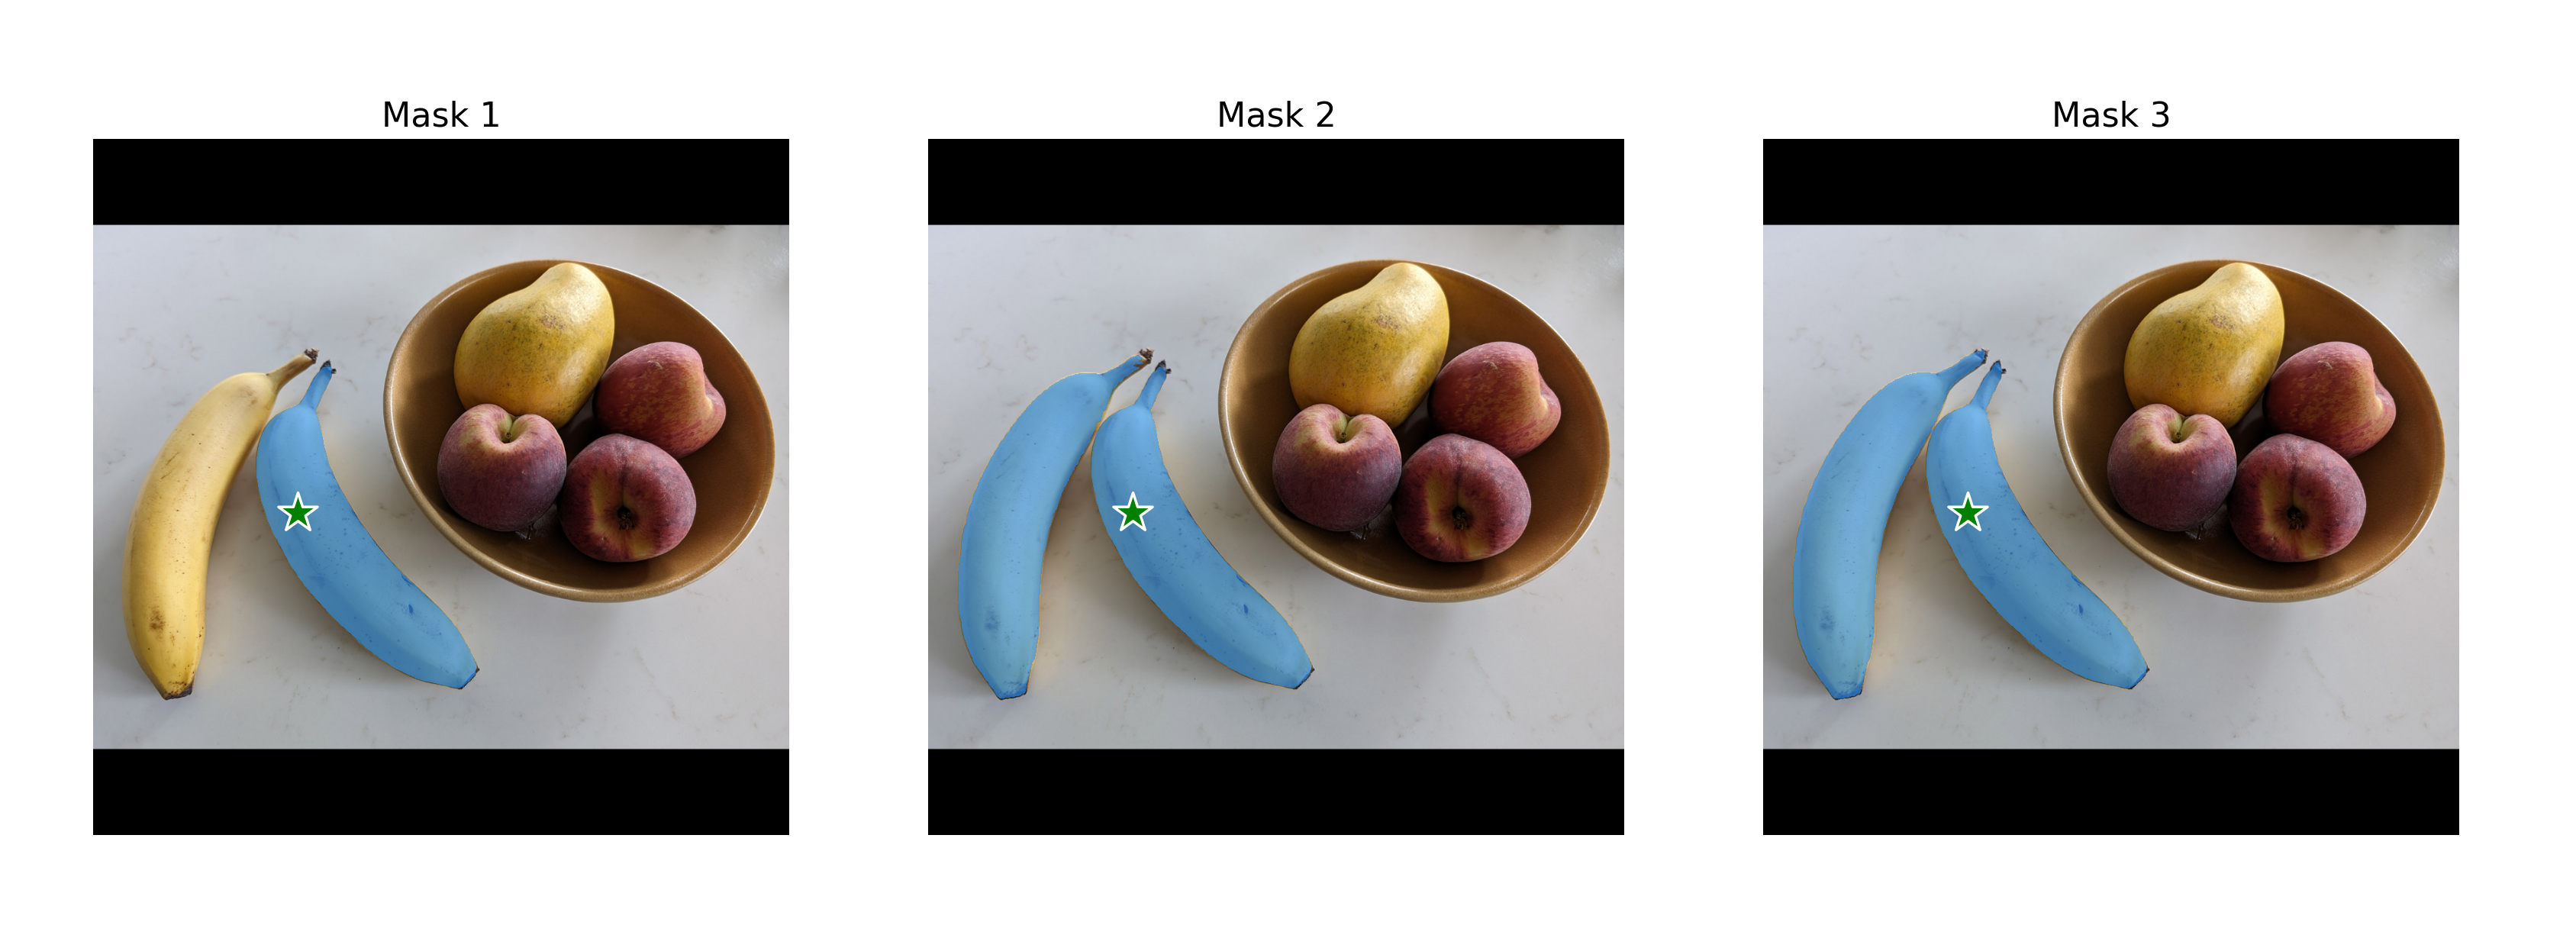
\includegraphics[width=\textwidth,height=0.6\textheight,keepaspectratio]{../../images/ch11/bananas_all_masks.c922b7a6.png}
            \caption{Các Mặt nạ thay thế của SAM}
        \end{figure}
    \end{columns}
\end{frame}

\begin{frame}[fragile]{Nhắc bằng Hộp giới hạn (Box Prompting)}
    \begin{columns}
        \column{0.5\textwidth}
        Cung cấp 1 hộp bao phủ trái xoài (Tọa độ Góc trên-trái và Góc dưới-phải).
        
\begin{lstlisting}[language=Python]
input_box = np.array([
    [520, 180], # Top-left corner
    [770, 420], # Bottom-right corner
])

outputs = model.predict(
    {
        "images": ops.expand_dims(img, axis=0),
        "boxes": ops.expand_dims(input_box, axis=(0, 1)),
    }
)
\end{lstlisting}
        
        \column{0.5\textwidth}
        \begin{figure}
            \centering
            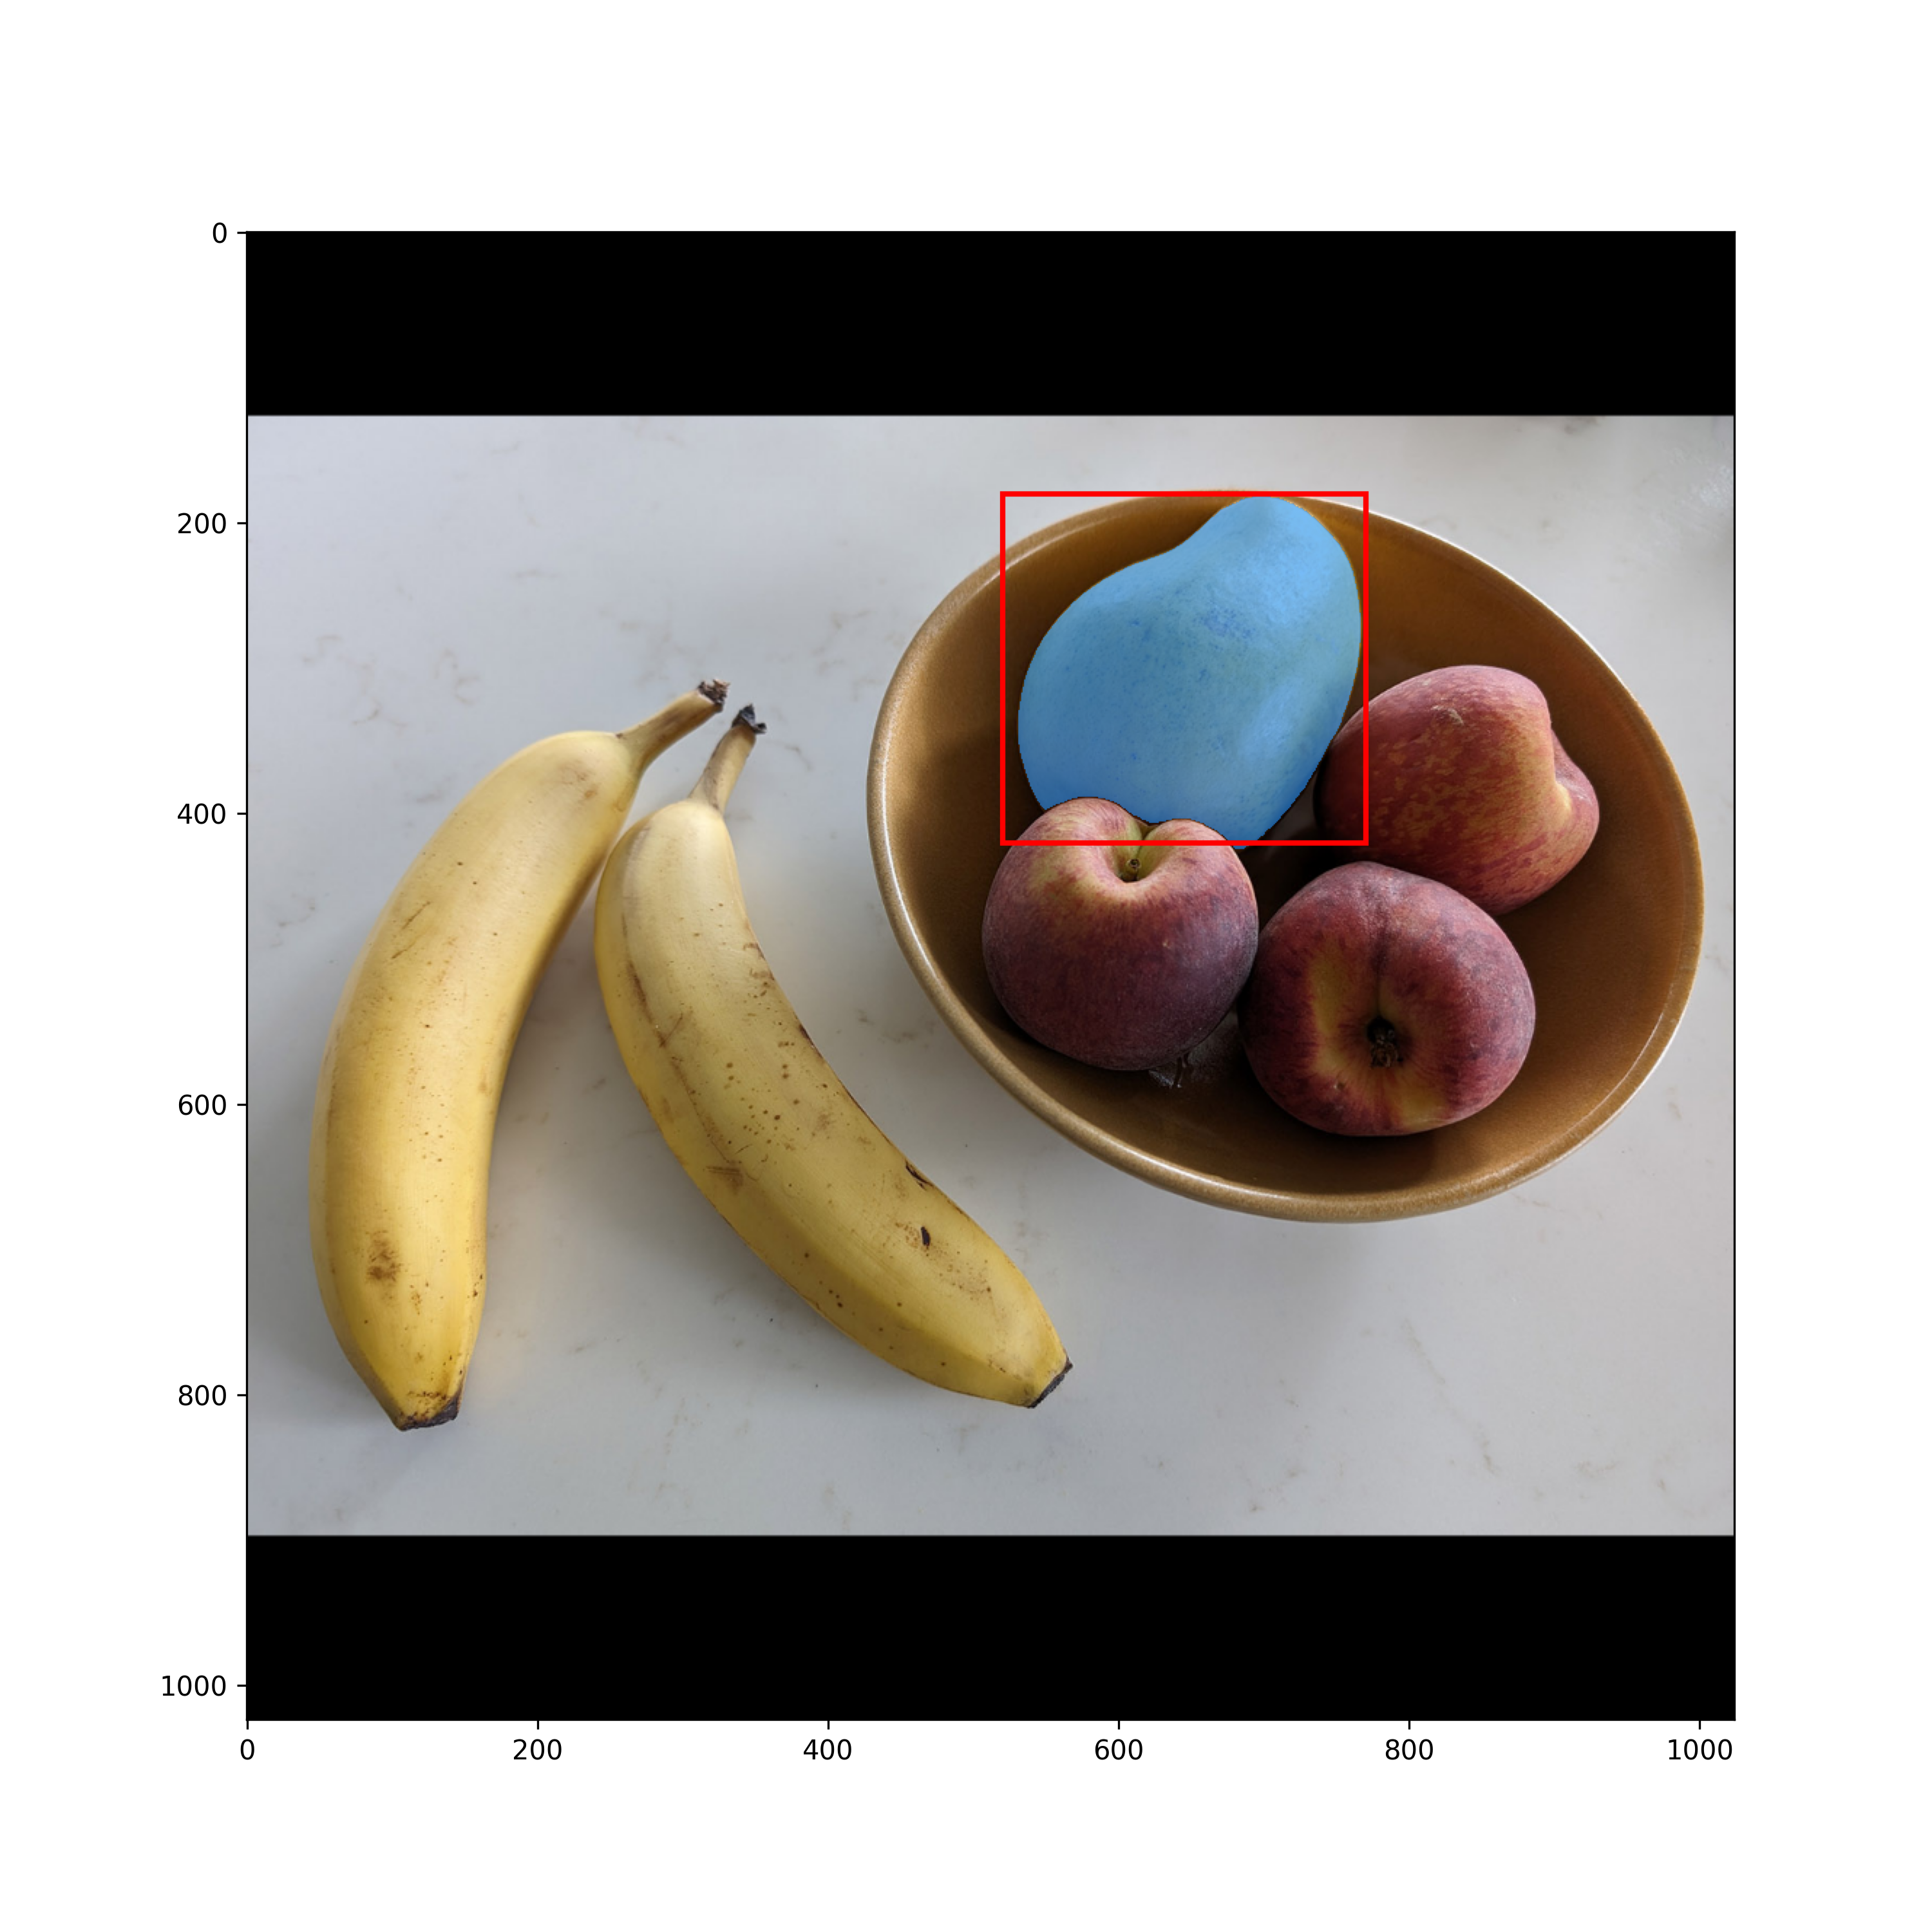
\includegraphics[width=\textwidth,height=0.5\textheight,keepaspectratio]{../../images/ch11/mango_segmented.2dfb0dae.png}
            \caption{SAM lập tức trả về Mặt nạ Xoài chính xác}
        \end{figure}
    \end{columns}
\end{frame}

\begin{frame}[fragile]{Nhắc bằng Điểm đơn (Single Point Prompting)}
    \begin{columns}
        \column{0.5\textwidth}
        Nhập đúng 1 tọa độ rơi vào quả Đào. (Nhãn $1$ nghĩa là Tiền cảnh, chọn cái này!)
        
\begin{lstlisting}[language=Python]
# Coordinates of our point
input_point = np.array([[580, 450]])

# 1 means foreground, 0 means background
input_label = np.array([1])

outputs = model.predict(
    {
        "images": ops.expand_dims(image, axis=0),
        "points": ops.expand_dims(input_point, axis=0),
        "labels": ops.expand_dims(input_label, axis=0),
    }
)
\end{lstlisting}
        
        \column{0.5\textwidth}
        \begin{figure}
            \centering
            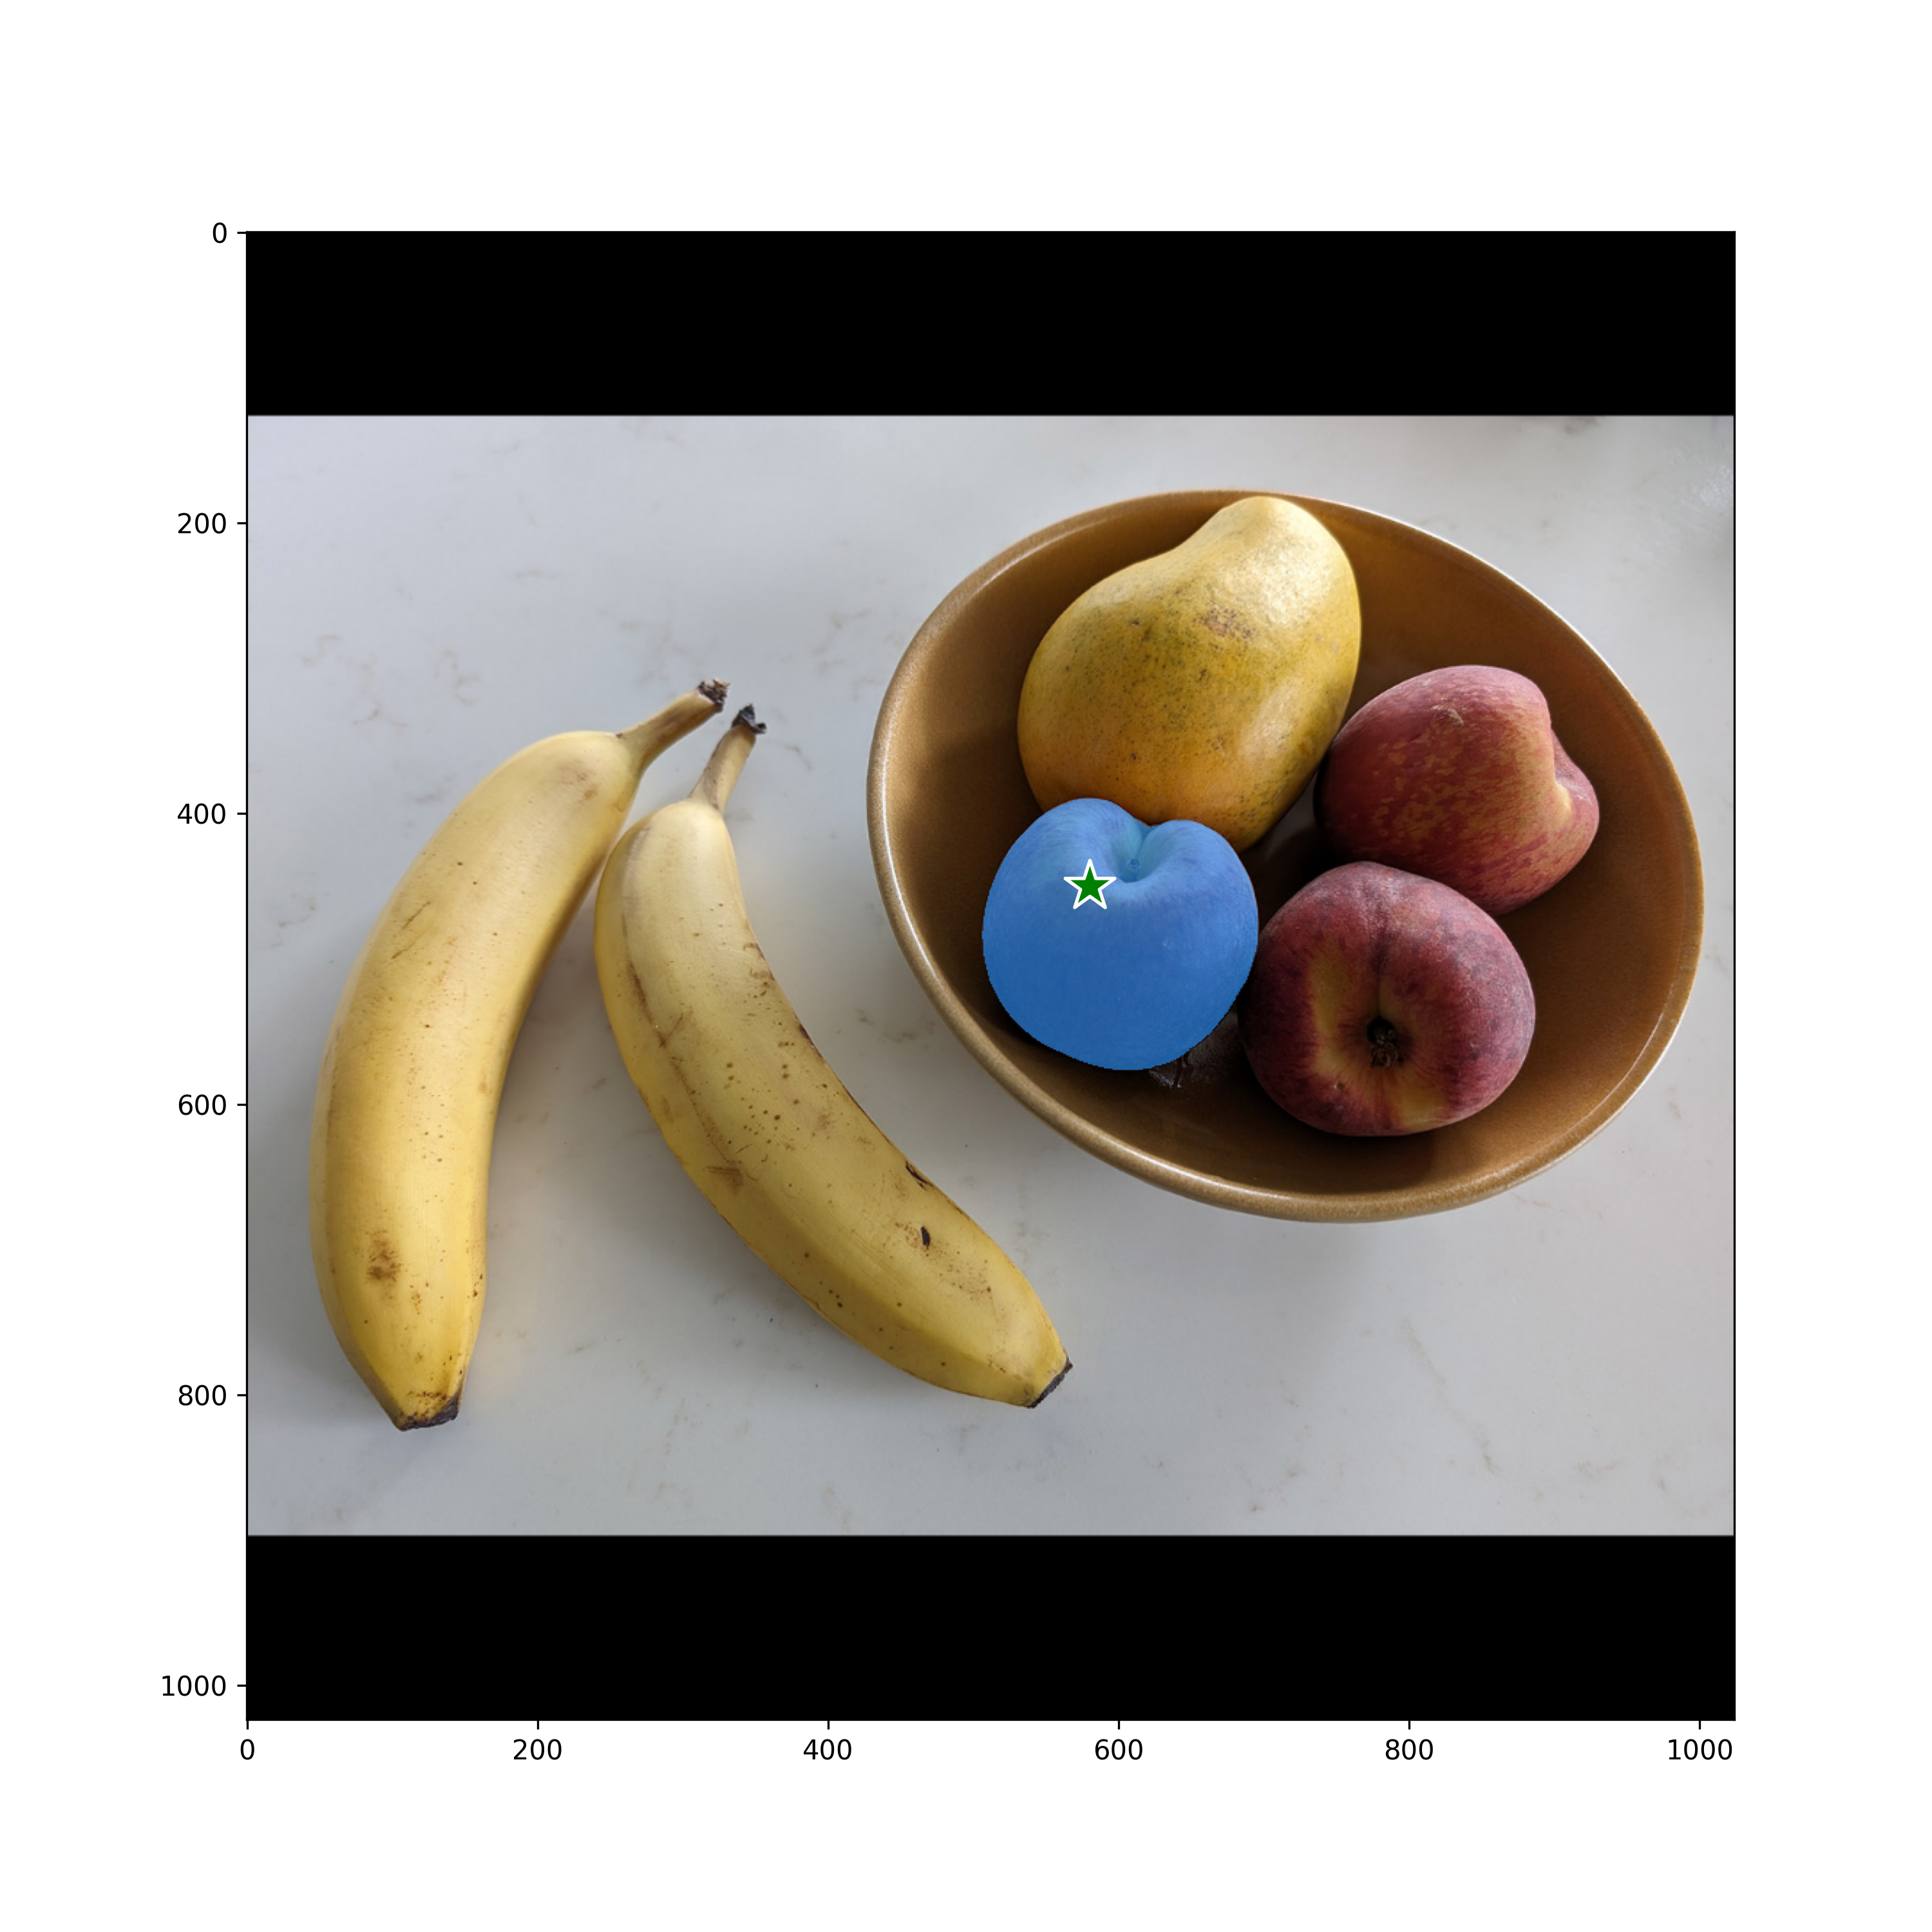
\includegraphics[width=\textwidth,height=0.5\textheight,keepaspectratio]{../../images/ch11/peach_segmented.333556ff.png}
            \caption{SAM lan truyền điểm đó thành Mặt nạ Đào}
        \end{figure}
    \end{columns}
\end{frame}

\begin{frame}{Sức mạnh nội suy của Point Prompt}
    \begin{columns}
        \column{0.5\textwidth}
        \begin{itemize}
            \item Tương tự, nếu ta truyền Tọa độ điểm của một quả Chuối bị khuất.
            \item Kể cả khi quả chuối bị che bởi bóng đổ hay trái cây khác, công cụ ViT khổng lồ của SAM vẫn nội suy (Interpolate) ra đường viền hoàn mỹ.
            \item Quá trình này diễn ra theo thời gian thực (Real-time) trong trình duyệt nhờ Mask Decoder siêu nhẹ.
        \end{itemize}
        
        \column{0.5\textwidth}
        \begin{figure}
            \centering
            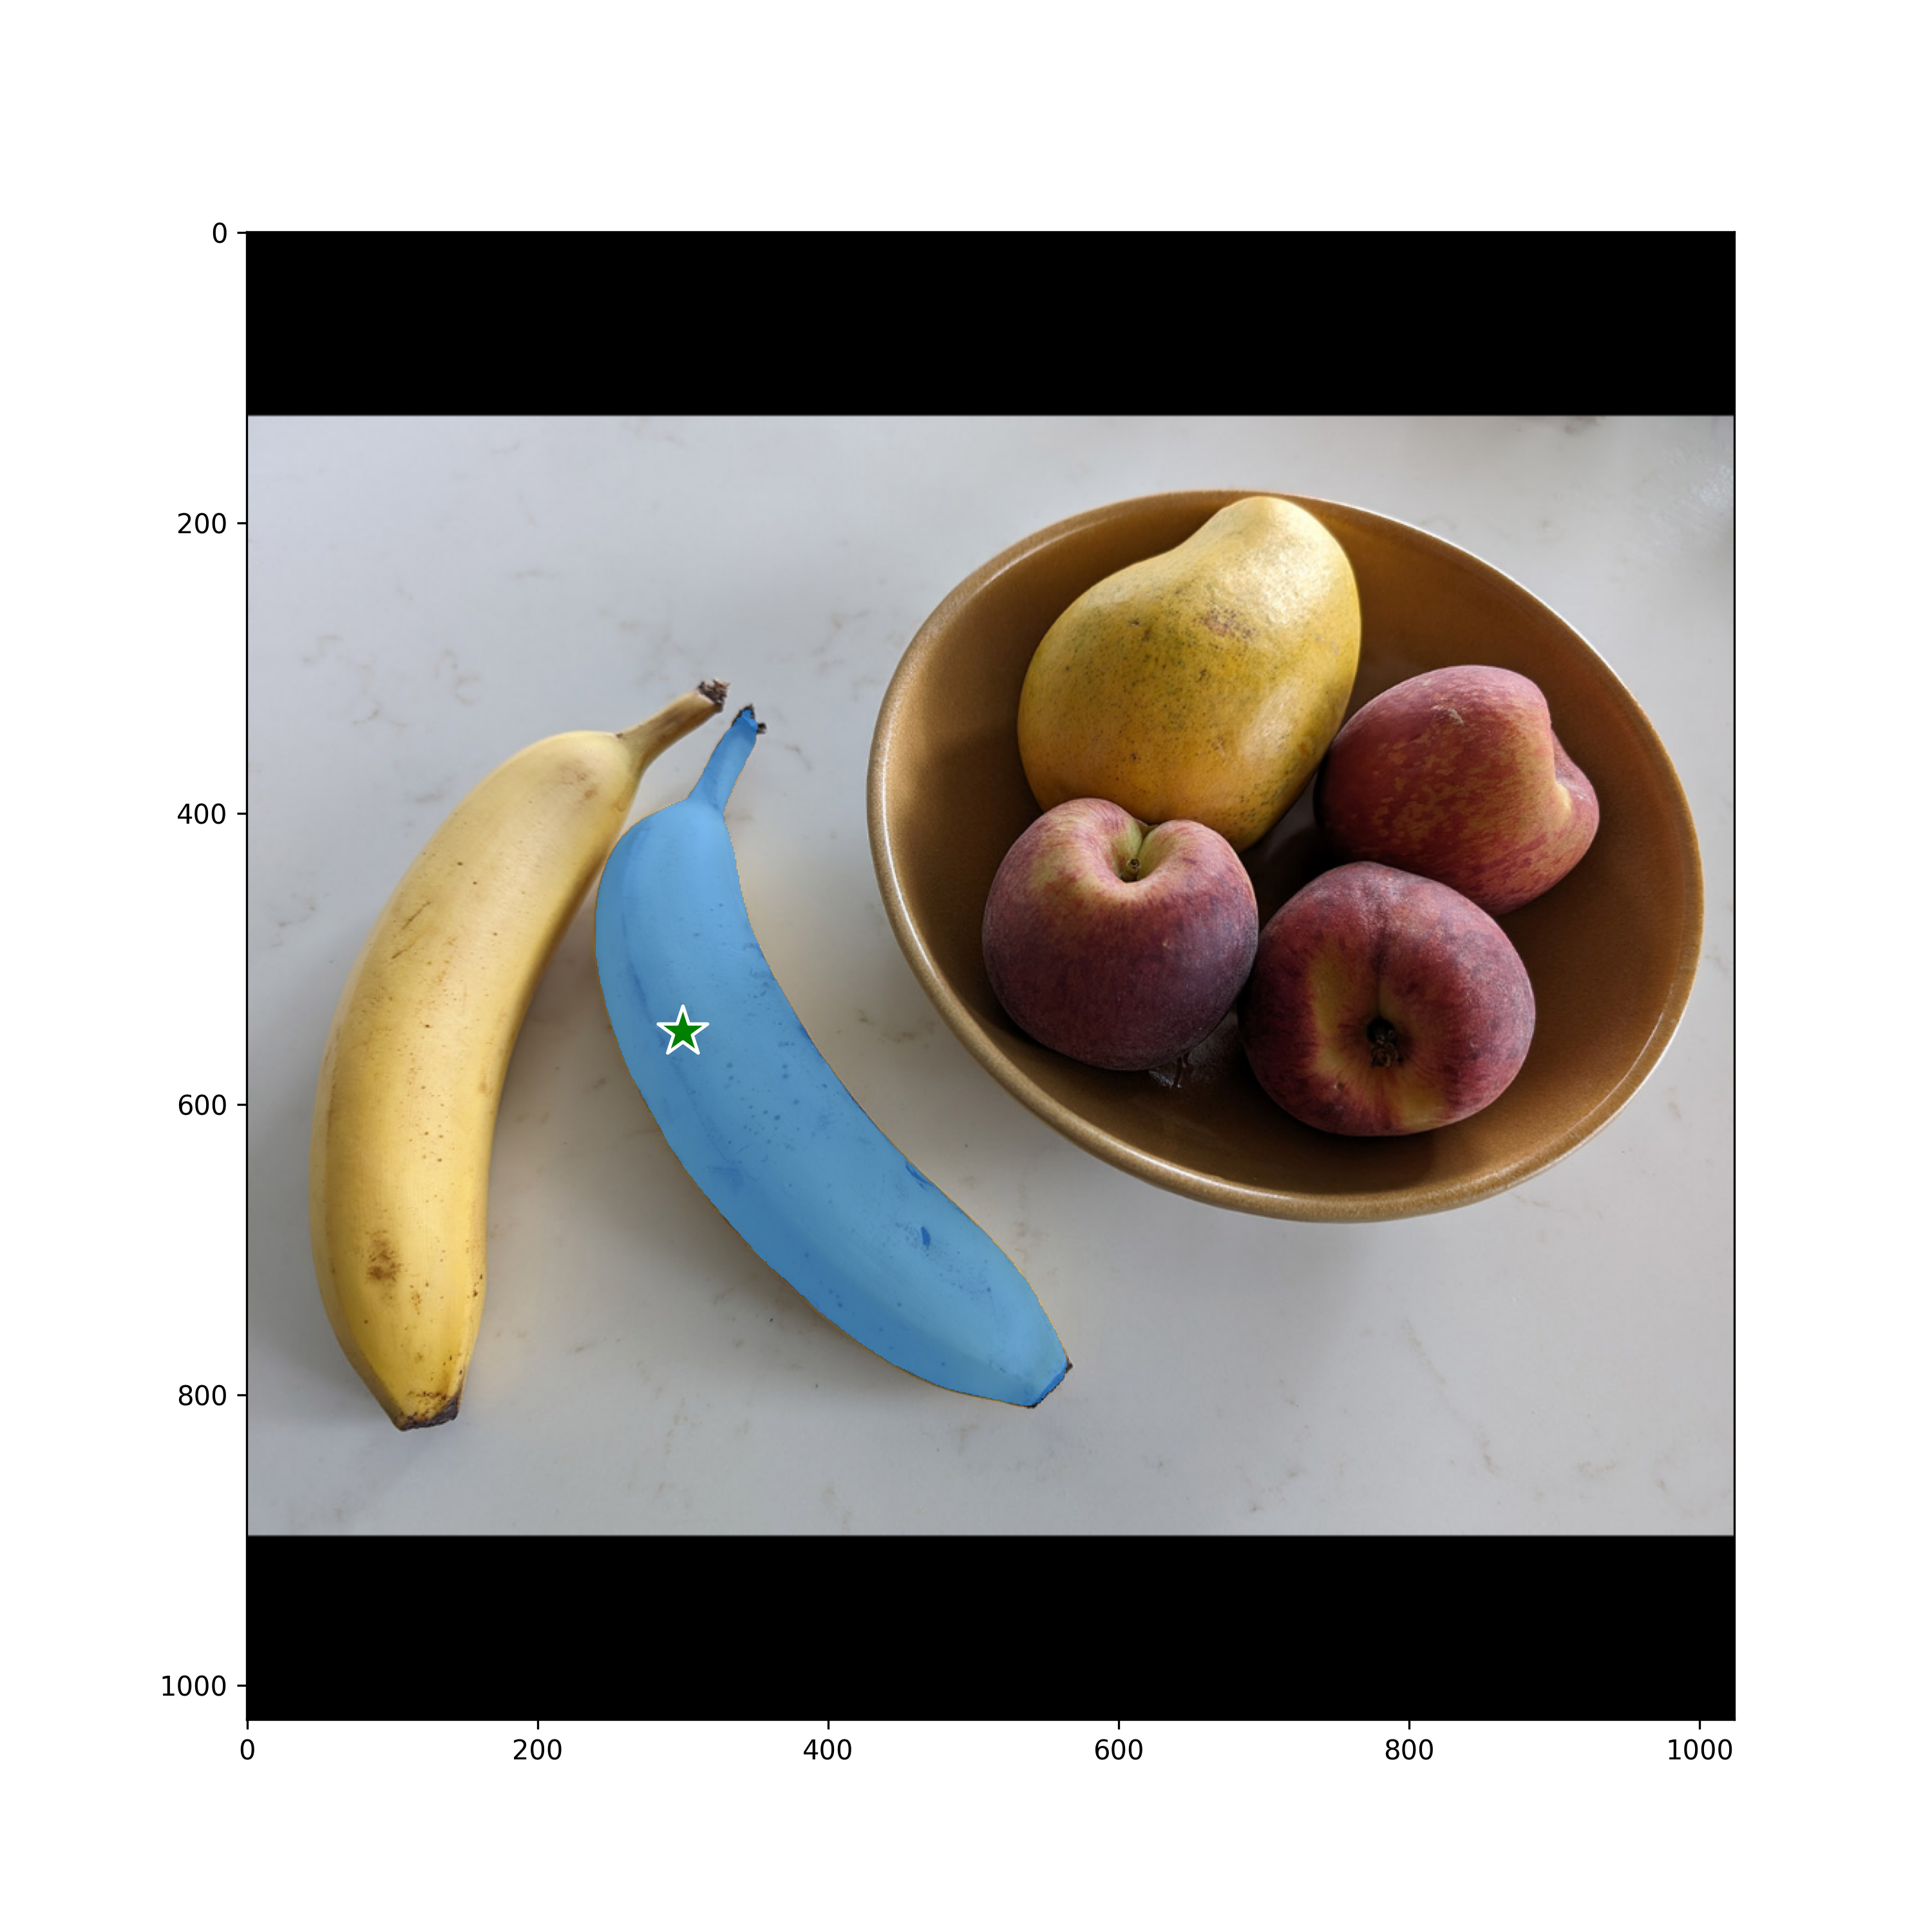
\includegraphics[width=\textwidth,height=0.6\textheight,keepaspectratio]{../../images/ch11/banana_segmented.8e0b3e81.png}
            \caption{Phân vùng Chuối bằng 1 Point Prompt}
        \end{figure}
    \end{columns}
\end{frame}

\section{Tổng kết}

\begin{frame}{Tổng kết Chương 11}
    \begin{itemize}
        \item \textbf{Image Segmentation} là bài toán tìm ranh giới chính xác đến từng pixel cho vật thể (Semantic, Instance, Panoptic).
        \item \textbf{U-Net \& Transposed Convolution:} Một mô hình kinh điển giải quyết phân vùng bằng kiến trúc Encoder (hạ phân giải để tìm Đặc trưng) và Decoder (tăng phân giải để Phục hồi không gian).
        \item \textbf{Segment Anything (SAM):} Đưa Computer Vision bước vào kỷ nguyên Foundation Model, cho phép phân vùng Zero-shot "Mọi thứ" chỉ bằng các gợi ý đơn giản (Point, Box, Text).
    \end{itemize}
\end{frame}

\end{document}
